\documentclass[a4paper, 11pt]{article}
\usepackage{fontspec}
\setmainfont{DejaVu Sans}
\setmonofont{DejaVu Sans Mono}
\usepackage[czech]{babel}

\AtBeginDocument{%
  \renewcommand{\figurename}{Obrázek}%
  \renewcommand{\tablename}{Tabulka}%
  \renewcommand{\contentsname}{Obsah}%
}
\usepackage[top=20mm, bottom=20mm, left=18mm, right=18mm]{geometry}
\usepackage{graphicx}
\usepackage[hidelinks, unicode, breaklinks=true]{hyperref}

% Prevent text overflow - allow more flexible line breaking
\tolerance=1000
\emergencystretch=2em
\hbadness=2000
\setlength{\hfuzz}{2pt}

% Allow URL breaks at any character
\makeatletter
\g@addto@macro{\UrlBreaks}{\UrlOrds}
\makeatother
\usepackage{xcolor}
\usepackage{titlesec}
\usepackage{enumitem}
\usepackage{booktabs}
\usepackage{tabularx}
\usepackage{longtable}
\usepackage{fancyhdr}
\usepackage{float}
\usepackage{parskip}
\usepackage{calc}
\usepackage{tocloft}

\setcounter{secnumdepth}{2}
\setcounter{tocdepth}{2}
\setlength{\cftsecnumwidth}{2.5em}
\setlength{\cftsubsecnumwidth}{3.5em}
\setlength{\cftsubsubsecnumwidth}{4.5em}
\setlength{\cftsubsecindent}{2.5em}

\definecolor{cblue}{HTML}{0C7FD6}
\definecolor{text2}{HTML}{4B5068}
\definecolor{text3}{HTML}{7C8198}
\definecolor{bg3}{HTML}{F0F1F4}

\titleformat{\section}{\Large\bfseries\color{black}}{\thesection\hspace{0.6em}}{0pt}{}[\vspace{-4pt}\textcolor{bg3}{\rule{\linewidth}{1pt}}]
\titleformat{\subsection}{\large\bfseries\color{black}}{\thesubsection\hspace{0.5em}}{0pt}{}
\titleformat{\subsubsection}{\normalsize\bfseries\color{text2}}{\thesubsubsection\hspace{0.5em}}{0pt}{}

\pagestyle{fancy}
\fancyhf{}
\fancyhead[L]{\small\textcolor{text3}{Multimodální systém pro sběr webových dat a AI analýzu}}
\fancyhead[R]{\small\textcolor{text3}{Tým APIčáci}}
\fancyfoot[C]{\small\textcolor{text3}{\thepage}}
\renewcommand{\headrulewidth}{0.4pt}

\newcommand{\docurl}[1]{\textcolor{cblue}{\url{#1}}}

\begin{document}

% ══════════ TITLE ══════════
\begin{titlepage}
\centering\vspace*{36mm}
{\huge\bfseries DOKUMENTACE\par}\vspace{10mm}
{\Large Multimodální systém pro sběr webových dat\\[4pt] a~AI analýzu (LLM + RAG)\par}
\vfill
{\normalsize Tým APIčáci\par}\vspace{10mm}
\end{titlepage}

\tableofcontents
\newpage

% ══════════ 1. ÚVOD ══════════
\section{Úvod}

Tento dokument popisuje návrh, architekturu a~způsob implementace systému \textit{Multimodální systém pro sběr webových dat a~AI analýzu (LLM + RAG)}, který bude vyvíjen třináctičlenným týmem APIčáci jako řešení pro zákazníka. Slouží jako referenční materiál pro vývojový tým a~zadavatele projektu.

Systém bude navržen pro zpracování obsahu z~různých typů zdrojů -- statických HTML stránek, dynamicky generovaného obsahu, PDF dokumentů i~vizuálního obsahu formou screenshot screeningu s~AI extrakcí. Bude implementován jako kontejnerizovaná aplikace nasazená na infrastruktuře e-INFRA CZ.

% ══════════ 2. KONTEXT ══════════
\subsection{Kontext projektu}

Projekt bude realizován v~rámci jednoho semestru jako týmový vývojový projekt určený k~reálnému nasazení. Důraz bude kladen nejen na funkčnost, ale také na stabilitu, rozšiřitelnost a~provozní udržitelnost řešení.

Architektura bude navržena jako modulární platforma organizovaná jako monorepo s~logickým oddělením frontendové aplikace, backendové služby a~modulů pro sběr, zpracování dat a~AI. Konkrétní technologický stack bude upřesněn v~průběhu fáze Rozpracování.

% ══════════ 3. CÍLE ══════════
\subsection{Cíl}

Hlavním cílem je navrhnout a~implementovat multimodální RAG systém (Retrieval-Augmented Generation) pro sběr webových dat, jejich indexaci a~analýzu pomocí AI. Odpovědi budou generovány s~dohledatelnými citacemi na zdrojové dokumenty, čímž se minimalizují halucinace.

Systém bude podporovat více strategií sběru dat (včetně screenshot screeningu a~AI extrakce) a~experimentální režim pro porovnávání embedding modelů a~přístupů RAG vs. no-RAG. Pro každý zdroj bude vyžadován právní titul a~retenční pravidla; při detekci CAPTCHA bude vytvořen incident bez obcházení ochrany.

\newpage
% ══════════ 4. USE CASE ══════════
\section{Use Case diagram}

Diagram případů užití zobrazuje interakce čtyř typů uživatelů (aktérů) se systémem. Každý aktér má specifickou sadu oprávnění definovaných prostřednictvím RBAC. Všichni aktéři dědí od společného předka \textit{Systémový uživatel} a~sdílejí use case \textit{Autentizace vůči systému}. Diagram je zobrazen na obr.~\ref{fig:usecase}.

\subsection{Aktéři}

\textbf{Systémový uživatel} bude abstraktním předkem všech rolí v~systému. Bude reprezentovat jakéhokoli autentizovaného uživatele a~sdílet use case Autentizace vůči systému.

\textbf{Standardní uživatel} bude koncovým uživatelem systému, který bude zadávat dotazy nad indexem a~přijímat odpovědi s~citacemi. Bude moci zvolit režim dotazování (RAG s~vyhledáním v~indexu nebo no-RAG pro přímou odpověď modelu). Nebude mít přístup ke správě zdrojů ani experimentům. Typickým uživatelem bude zaměstnanec, výzkumník nebo student.

\textbf{Analytik} bude uživatel se zaměřením na evaluaci a~experimenty. Bude moci spouštět experimenty, porovnávat různé přístupy k~vyhledávání, specifikovat testovací datasety dotazů a~přijímat automatizované reporty s~výsledky. Typickým uživatelem bude data scientist nebo výzkumník.

\textbf{Kurátor} bude správce zdrojů dat. Bude přidávat nové webové zdroje ke sběru, dokládat právní tituly a~licence, nastavovat pravidla sběru (frekvence, hloubka, strategie) a~řešit CAPTCHA incidenty. Kurátor bude specializací Systémového uživatele (generalizace v~diagramu). Typickým uživatelem bude datový knihovník nebo správce obsahu.

\textbf{Administrátor} bude mít plný přístup ke konfiguraci systému. Bude spravovat uživatele a~role, systémové nastavení, retenční politiky a~přístupové údaje ke službám. Bude moci řešit CAPTCHA incidenty (sdílený use case s~Kurátorem). Typickým uživatelem bude DevOps nebo systémový administrátor.

\subsection{Přehled use cases}

Systém definuje dvanáct případů užití pokrývajících celý životní cyklus práce s~daty -- od přihlášení přes zadávání dotazů a~správu zdrojů až po spouštění experimentů a~administraci systému. Každý případ užití je přiřazen konkrétní roli, přičemž některé jsou sdílené nebo tvoří součást nadřazeného use case prostřednictvím vztahu \texttt{<<zahrnuje>>}. Přehled use cases a jejich aktérů je uveden v tab.~\ref{tab:usecases}.

\subsection{Vztahy v diagramu}

Diagram využívá vztah \texttt{<<zahrnuje>>} (include) pro vyjádření nedílné součásti jiného use case. Například \textit{Zadání dotazu} zahrnuje \textit{Obdržení odpovědi s~citacemi} a~\textit{Volba režimu dotazování}, protože tyto kroky budou vždy součástí zpracování dotazu. Podobně \textit{Přidání zdroje pro sběr dat} zahrnuje \textit{Doložení povolení/licencí} a~\textit{Nastavení pravidel sběru dat}. Generalizace (plná šipka) znázorňuje, že Kurátor je specializací Systémového uživatele.

\begin{figure}[H]
\centering
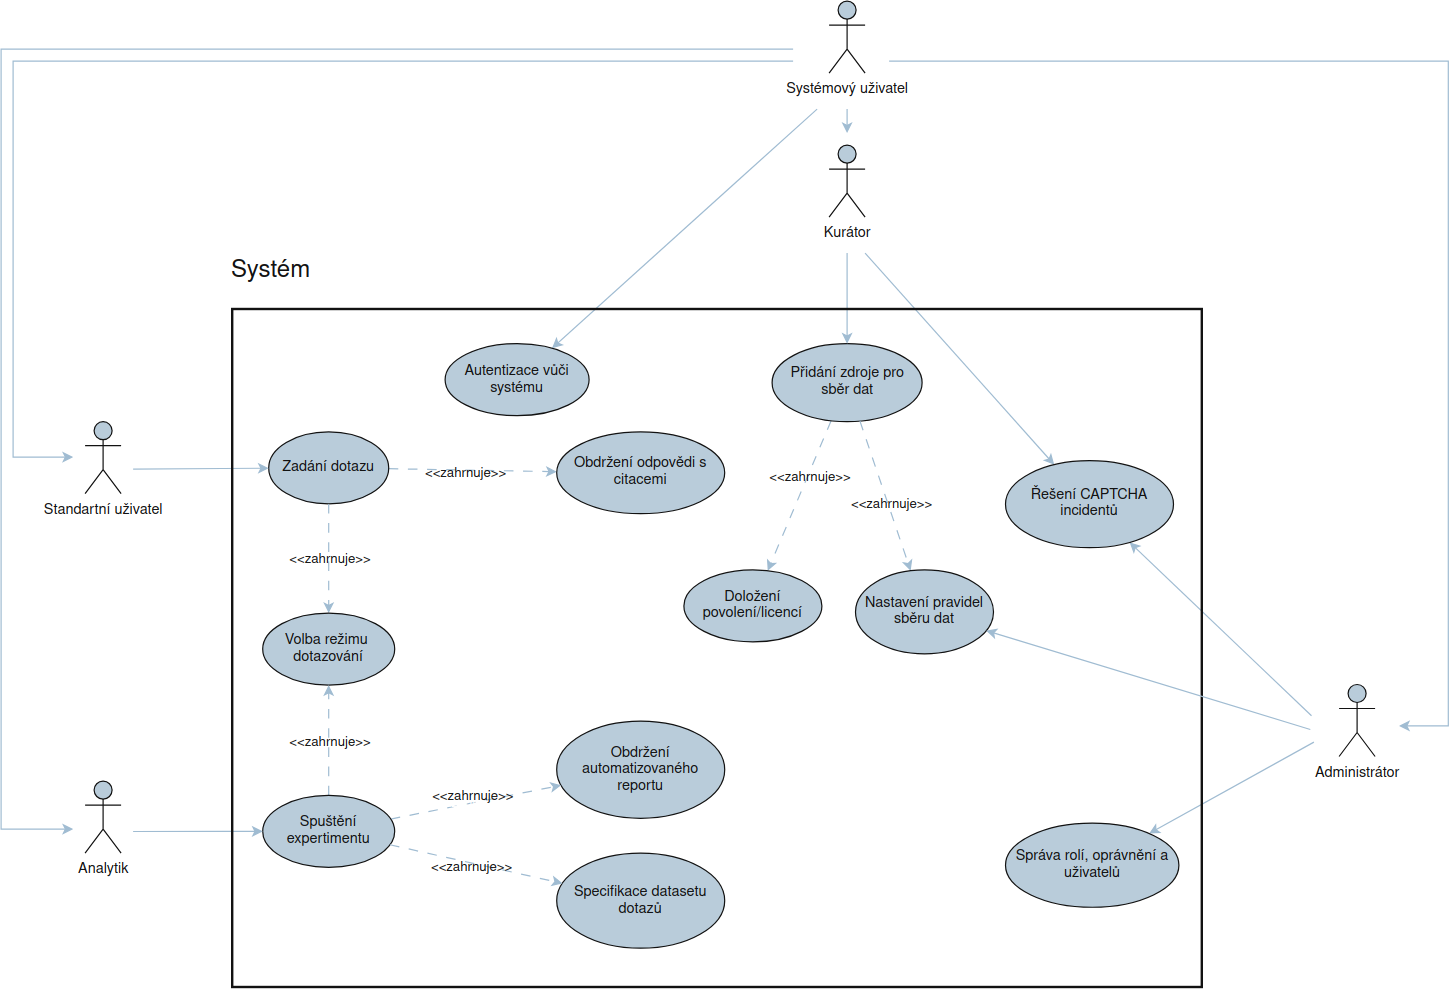
\includegraphics[width=0.88\textwidth]{usecase_trimmed.png}
\caption{Use Case diagram -- role a jejich interakce se systémem}
\label{fig:usecase}
\end{figure}

\begin{table}[H]
\centering\small
\begin{tabularx}{\textwidth}{l l X}
\toprule
\textbf{Use case} & \textbf{Aktér} & \textbf{Popis} \\
\midrule
Autentizace vůči systému & Systémový uživatel & Přihlášení do systému. Sdíleno všemi rolemi. \\
\addlinespace
Zadání dotazu & Std. uživatel & Zadání dotazu v~přirozeném jazyce přes webové rozhraní nebo API. \\
\addlinespace
Volba režimu dotazování & Std. uživatel & Výběr RAG nebo no-RAG. Zahrnuto (<<zahrnuje>>) v~zadání dotazu. \\
\addlinespace
Obdržení odpovědi s~citacemi & Std. uživatel & Odpověď AI s~citacemi na zdrojové dokumenty. Zahrnuto v~zadání dotazu. \\
\addlinespace
Spuštění experimentu & Analytik & A/B test embeddingů nebo srovnání RAG vs. no-RAG. \\
\addlinespace
Specifikace datasetu dotazů & Analytik & Definice testovacích dotazů a~ground truth. Zahrnuto v~experimentu. \\
\addlinespace
Obdržení aut. reportu & Analytik & Výsledky hodnocení kvality vyhledávání. Zahrnuto v~experimentu. \\
\addlinespace
Přidání zdroje pro sběr dat & Kurátor & Registrace nového webu s~pravidly sběru. \\
\addlinespace
Doložení povolení/licencí & Kurátor & Právní titul ke zdroji. Zahrnuto v~přidání zdroje. \\
\addlinespace
Nastavení pravidel sběru & Kurátor & Frekvence, hloubka, strategie, retence. Zahrnuto v~přidání zdroje. \\
\addlinespace
Řešení CAPTCHA incidentů & Kurátor, Admin & Vyřešení incidentu, doplnění chybějících dat. \\
\addlinespace
Správa rolí a~uživatelů & Administrátor & Správa přístupů, systémové nastavení a~přístupové údaje. \\
\bottomrule
\end{tabularx}
\caption{Přehled use cases a jejich aktérů}
\label{tab:usecases}
\end{table}

\newpage
% ══════════ 5. ARCHITEKTURA ══════════
\section{Architektura}
\label{sec:architektura}

Architektura bude organizována do šesti částí, kterými budou proudit data -- od uživatelského požadavku přes zpracování a~AI služby až po úložiště a~infrastrukturu. Systém bude koncipován jako modulární distribuovaná aplikace, kde jednotlivé komponenty budou komunikovat prostřednictvím API, front zpráv a~sdílených úložišť. Celkový přehled je zachycen na obr.~\ref{fig:architektura}.

Následující podsekce popisují jednotlivé vrstvy architektury s~detailem na konkrétní komponenty, technologie a~jejich vzájemné propojení.

\begin{figure}[H]
\centering
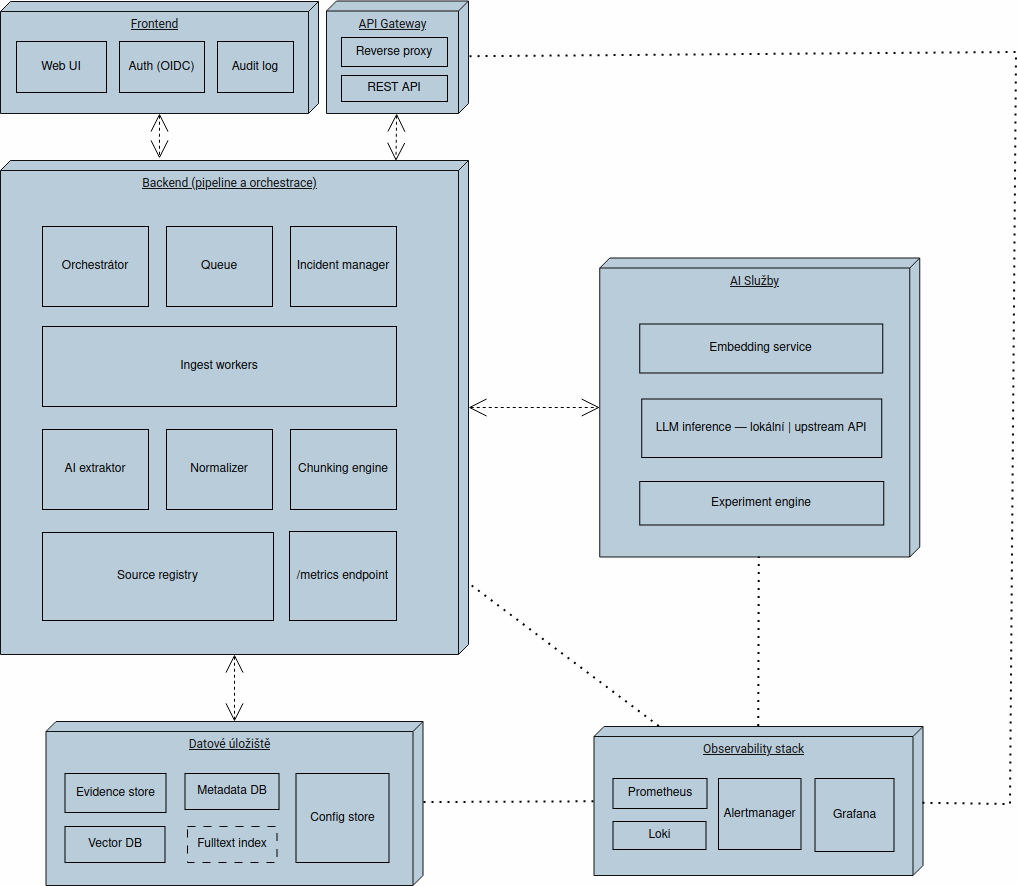
\includegraphics[width=0.82\textwidth]{komponentovy.png}
\caption{Komponentový diagram -- přehled architektury systému}
\label{fig:architektura}
\end{figure}

\subsection{Uživatelská vrstva a~API Gateway}

Webové uživatelské rozhraní bude implementováno ve frameworku Vue~3~\cite{vuejs, typescript} s~jazykem TypeScript. Bude sloužit pro přihlášení, zadávání dotazů, prohlížení odpovědí s~citacemi, administraci zdrojů a~monitoring stavu systému. Komunikace s~backendem bude probíhat přes REST API.

Autentizace a~autorizace bude zajištěna systémem \textbf{Keycloak}~\cite{keycloak} jako centrálním Identity Providerem (IdP) pro celý systém. Aplikace (frontend + FastAPI backend) budou využívat standardní OIDC flow -- uživatel se přihlásí přes Google účet, Keycloak vydá JWT token, backend ověří jeho podpis a~přidělí roli (Administrátor, Kurátor, Analytik, Standardní uživatel).

Interní nástroje infrastruktury, které nativně OIDC nepodporují (Grafana, RabbitMQ Management UI, Qdrant Web UI, Prometheus aj.), budou chráněny vzorem \textbf{Forward Authentication} na úrovni reverzní proxy. Traefik~\cite{traefik} \texttt{forwardAuth} middleware (resp. NGINX Ingress~\cite{nginxingress} anotace \texttt{auth-url}) bude každý příchozí požadavek před předáním službě ověřovat prostřednictvím instance \textbf{oauth2-proxy}~\cite{oauth2proxy}, která validuje session vůči Keycloaku. Tímto způsobem bude vynuceno jednotné přihlášení (SSO) pro libovolnou interní službu bez nutnosti její modifikace.

Každá akce v~systému bude zaznamenávána do auditního logu uloženého v~databázi PostgreSQL~\cite{postgresql} -- přihlášení, dotazy, exporty, změny konfigurace a~incidenty.

REST API bude postaveno na frameworku FastAPI~\cite{fastapi} (Python), který bude automaticky generovat OpenAPI dokumentaci a~zajišťovat rate limiting. Backend bude implementovat business logiku, komunikovat s~databází a~koordinovat AI moduly.

Reverzní proxy bude přijímat požadavky z~internetu, šifrovat spojení (HTTPS) a~směrovat na správné interní služby. V~MVP fázi bude použit Traefik, v~produkčním Kubernetes~\cite{kubernetes} prostředí NGINX Ingress nebo Traefik (dle konfigurace Rancher~\cite{rancher} clusteru). TLS certifikáty budou získávány automaticky od Let's Encrypt přes cert-manager~\cite{certmanager}. V~prostředí CERIT-SC~\cite{ceritk8s} Kubernetes bude k~dispozici předkonfigurovaný \texttt{letsencrypt-prod} ClusterIssuer.

Architektura bude rozlišovat několik oddělených virtuálních sítí: aplikační síť pro komunikaci mezi frontendem, backendem, orchestrátorem a~workery, síť úložiště pro komunikaci s~databázemi a~objektovým úložištěm a~observability síť pro monitoring a~logování. Tato vrstva je zachycena na obr.~\ref{fig:layer1}.

\begin{figure}[H]
\centering
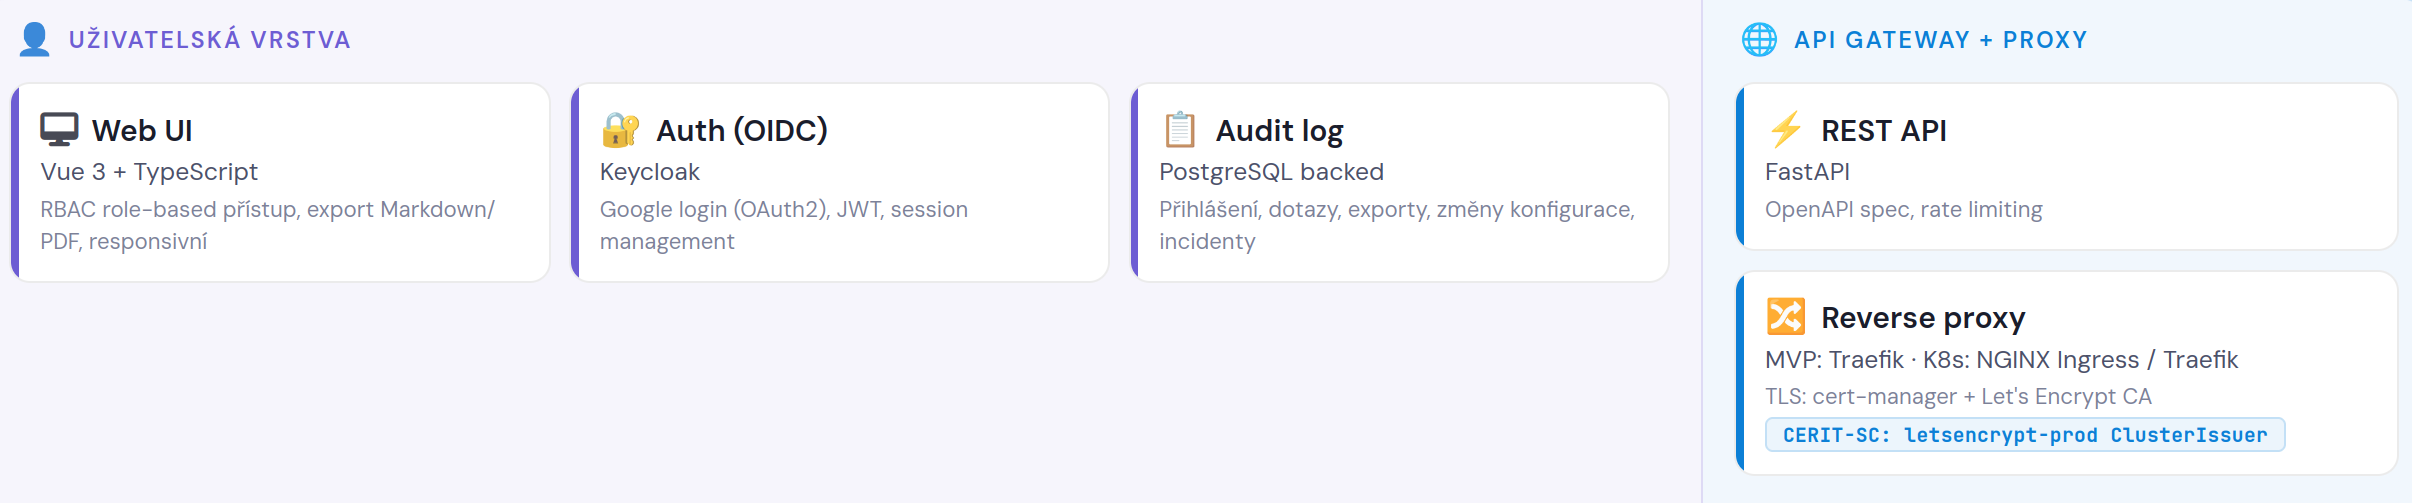
\includegraphics[width=\textwidth]{layer1.png}
\caption{Uživatelská vrstva a API Gateway}
\label{fig:layer1}
\end{figure}

\newpage
\subsection{Backend -- pipeline a orchestrace + AI služby}

\subsubsection{Orchestrátor, fronta a incident management}

Orchestrátor (Prefect~\cite{prefect} nebo Temporal) bude řídit celý workflow: bude plánovat stahování zdrojů, zajišťovat retry při selhání a~koordinovat pořadí operací. Při spuštění ingest úlohy vytvoří záznam a~zařadí ji do fronty zpráv RabbitMQ~\cite{rabbitmq}. Worker procesy budou odebírat úlohy z~fronty a~provádět jednotlivé kroky pipeline. Oddělení CPU a~GPU workerů umožní efektivní využití výpočetních prostředků.

Incident manager bude automaticky detekovat CAPTCHA a~další překážky při sběru dat. Při detekci uloží důkaz (screenshot stránky s~CAPTCHA), zapíše incident do databáze a~zařadí do fronty pro řešení Kurátorem nebo Administrátorem. Po vyřešení incidentu systém automaticky zopakuje ingest a~doplní chybějící dokumenty do indexu. Dashboard incidentů bude zobrazovat počty, zdroje a~trendy.

\subsubsection{Ingest workers -- multimodální fallback řetězec}

Klíčová inovace systému. Každý zdroj bude stahován pomocí řetězce strategií s~automatickým přechodem na další, pokud předchozí nedá dostatečný obsah (quality threshold) nebo selže: (1) API/Feed -- strukturované rozhraní, nejlepší kvalita, (2) HTML fetch + parse -- extrakce ze zdrojového kódu s~boilerplate removal, (3) Rendered DOM pomocí Playwright~\cite{playwright} -- plný prohlížeč, JavaScript rendering, DOM snapshot, (4) Screenshot screening -- full-page snímek a~AI extrakce textu a~struktury z~obrázku, (5) Upstream AI provider -- komerční AI služba jako záloha.

Každý krok pipeline bude generovat metadata ukládaná do databáze. Součástí bude vyhodnocení kvality extrahovaného obsahu -- pokud kvalita nedosáhne definovaného prahu, systém automaticky přejde na další strategii.

\subsubsection{AI extraktor, normalizace a chunking}

AI extraktor bude používat model Qwen2.5-VL-7B~\cite{qwen25vl} -- open-source vision-language model, který z~obrázku stránky rozpozná text (OCR), identifikuje nadpisy, odstavce, tabulky a~odstraní navigační prvky, patičky a~cookie bannery. Model dobře zvládá češtinu a~poběží lokálně na GPU (T4 16GB+ / L40 48GB).

Normalizer vytvoří ze stažených dat jednotný formát dokumentu (Canonical Document: title, sections, tables, metadata, citations) a~bude detekovat duplicity pomocí hash obsahu a~shingling. Bude podporovat verzování s~možností rebuild a~rollback. Chunking engine pak dokument rozřeže na menší kousky s~konfigurovatelnou velikostí, překryvem a~sémantickým dělením dle nadpisů. Tabulky a~layout bloky ze screenshotů budou mít samostatné chunky.

Source registry bude evidovat všechny zdroje -- URL, pravidla sběru, právní titul, retenční pravidla.

\subsubsection{AI služby -- embedding, LLM inference a experimenty}

Embedding service bude převádět chunky na vektory čísel reprezentující jejich význam. Model BGE-M3~\cite{bgem3} je multilingvální (čeština), bude produkovat dense i~sparse vektory, což umožní přesnější vyhledávání zejména v~kombinaci s~hybridním retrievalem. Bude podporovat A/B testy embeddingů. GPU požadavky: T4 16GB.

Volba inference enginu pro lokální LLM zatím není finálně rozhodnuta -- zvažují se dvě možnosti:

\textbf{llama.cpp}~\cite{llamacpp} je nízkoúrovňový, vysoce optimalizovaný engine pro kvantizované modely ve formátu GGUF. Nabízí maximální kontrolu nad parametry inference (GPU layers, batch size, context length) a~minimální overhead. HTTP server s~OpenAI-kompatibilním API je k~dispozici, ale vyžaduje ruční správu modelů a~konfiguraci. Je vhodný zejména pro prostředí HPC (MetaCentrum~\cite{metacentrum} PBS joby), kde nelze provozovat persistentní démon.

\textbf{Ollama}~\cite{ollama} je nadstavba nad llama.cpp poskytující OpenAI-kompatibilní REST API, automatickou správu modelů (\texttt{ollama pull}), detekci GPU a~jednoduchou konfiguraci. Výrazně zkracuje čas potřebný ke zprovoznění inference služby a~usnadňuje integraci -- jakýkoliv klient OpenAI SDK funguje bez úprav. Mírně vyšší overhead oproti čistému llama.cpp. \textbf{S~ohledem na časový rozsah projektu (jeden semestr) se Ollama jeví jako pragmatičtější volba}; finální rozhodnutí bude učiněno v~průběhu fáze Konstrukce.

Primárním modelem bude Llama 3.3 70B (Q4\_K\_M, cca 40~GB VRAM), alternativou Qwen2.5-72B pro silnější výkon v~češtině a~lehčím modelem Mistral Small 3.1 24B pro rychlejší odpovědi. Bude podporovat RAG i~no-RAG režim se strict grounding. GPU požadavky: L40S 48GB (alfrid cluster) / DGX H100 80GB.

Pro srovnání kvality a~jako záložní řešení bude systém podporovat komerční AI služby: Anthropic Claude (Opus/Sonnet), Google AI Studio (Gemini) a~OpenAI (GPT-4o/GPT-4.1).

Experiment engine bude umožňovat systematické testování kvality. Metriky retrieval: Recall@k, MRR, nDCG. Metriky odpovědi: latence, coverage citacemi, detekce tvrzení bez opory. Automatizované reporty budou srovnávat minimálně 2 embeddingy a~režim RAG vs. no-RAG. Schéma backendu je zobrazeno na obr.~\ref{fig:layer2}.

\begin{figure}[H]
\centering
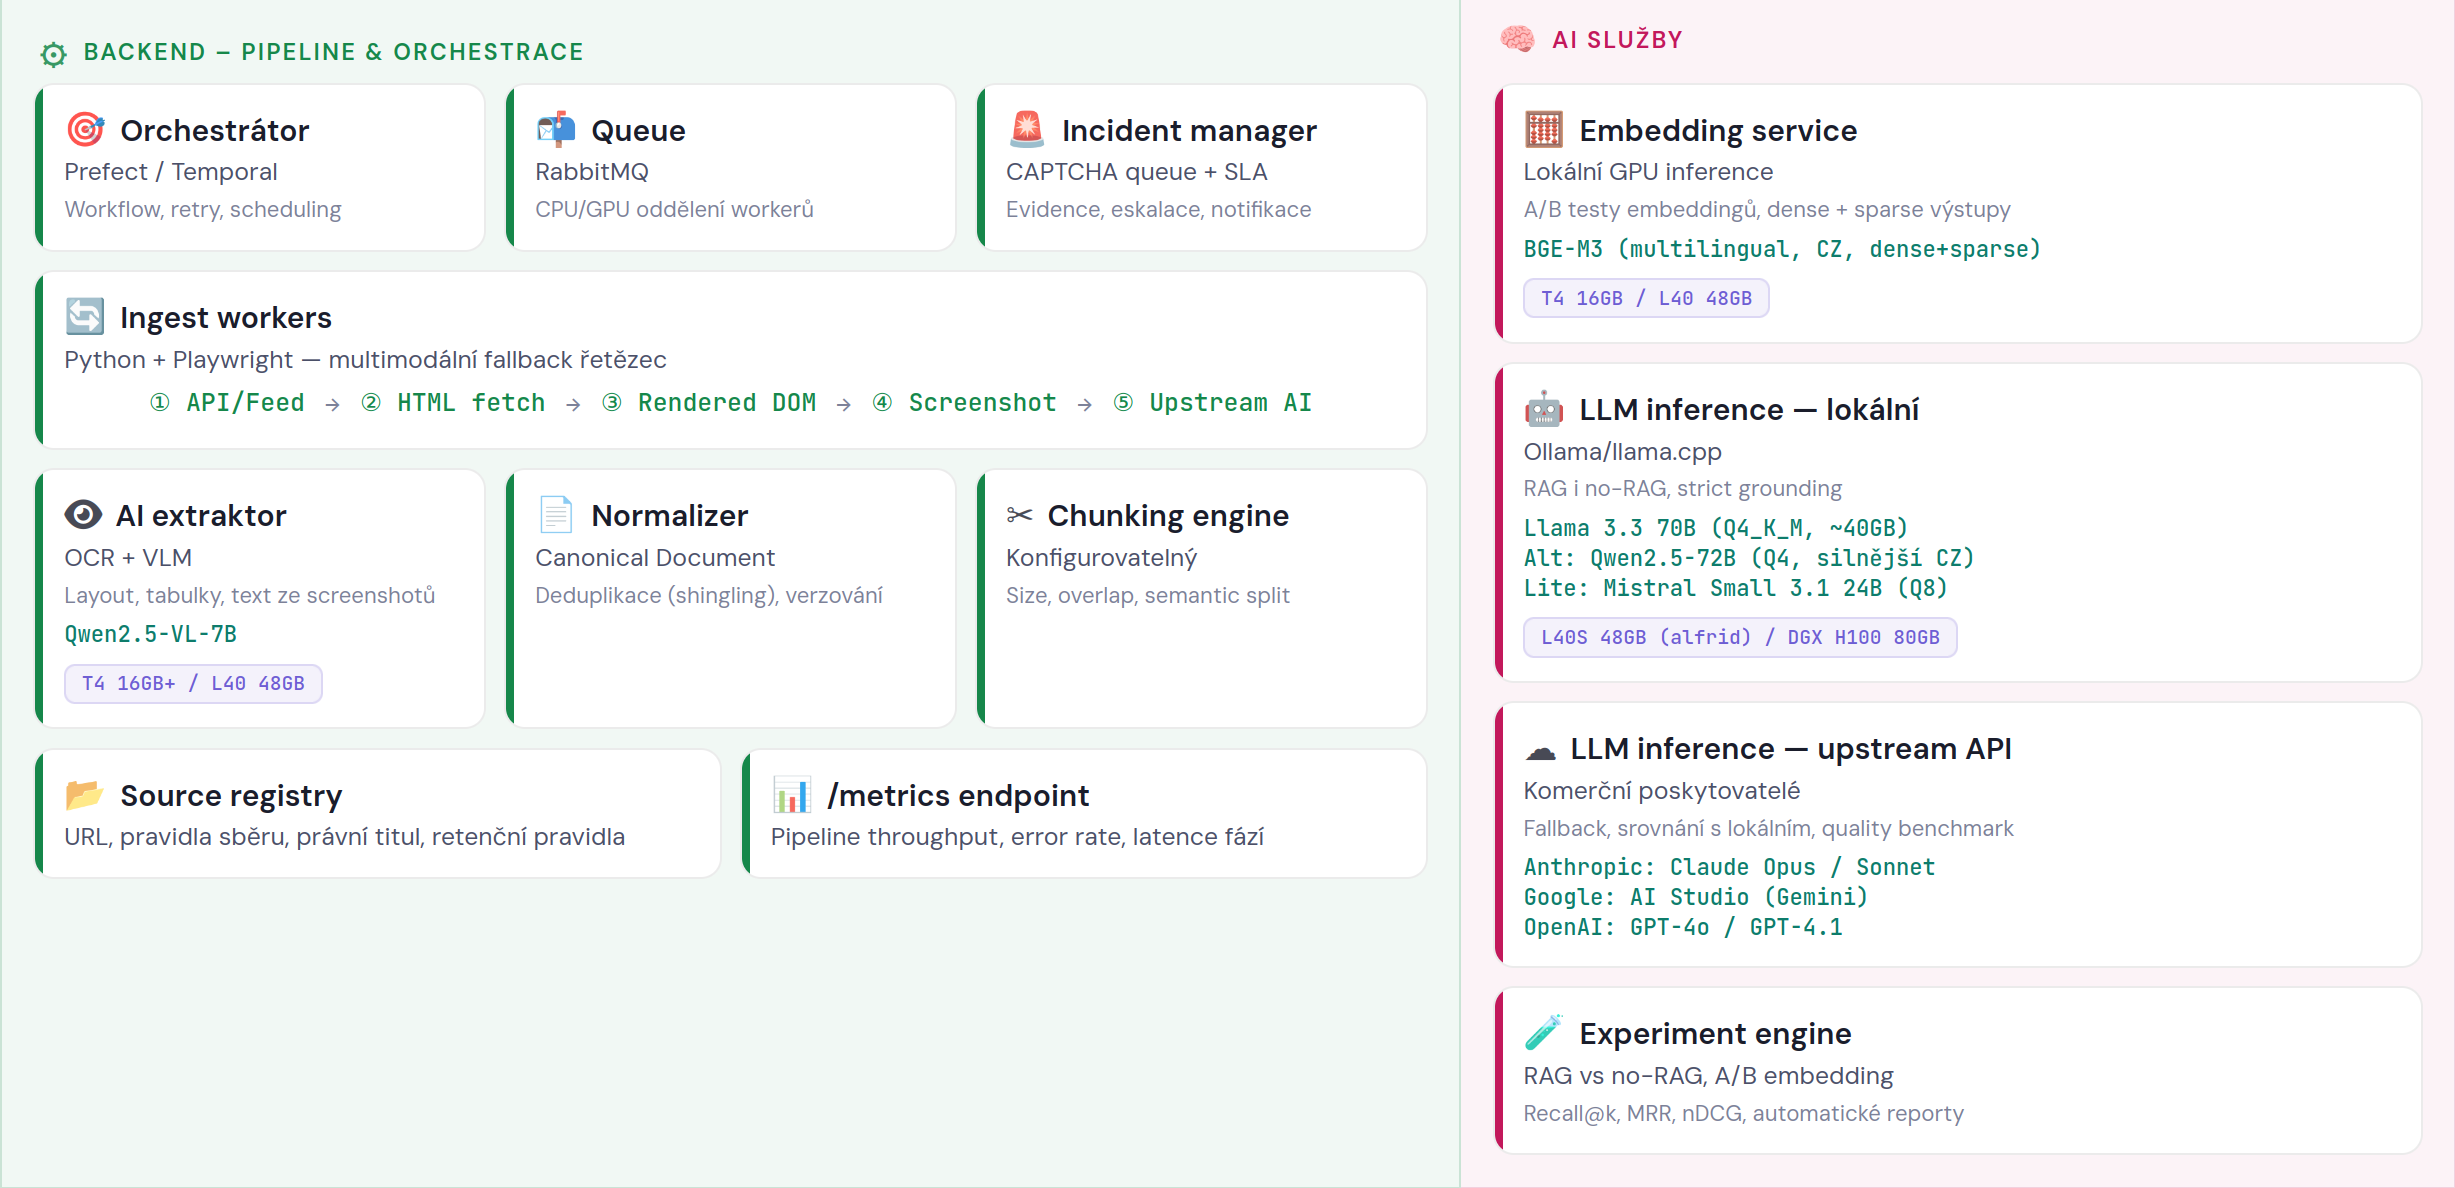
\includegraphics[width=\textwidth]{layer2.png}
\caption{Backend pipeline, orchestrace a AI služby}
\label{fig:layer2}
\end{figure}

\newpage
\subsection{Datové úložiště}

Evidence store bude S3-kompatibilní objektové úložiště (Ceph, MinIO~\cite{minio} nebo Garage) pro důkazní artefakty: full-page screenshoty se SHA-256 hash, DOM snapshoty, stažená HTML a~PDF, bounding box citace, CAPTCHA evidence, upstream AI surové odpovědi a~síťová metadata. Versioning a~retenční pravidla budou konfigurovatelné per zdroj. V~produkci bude možné využít CESNET S3 storage nebo MinIO Operator na Kubernetes.

Metadata DB (PostgreSQL) bude uchovávat vše strukturované: Source registry, IngestJob stav a~historii, Document verze s~quality\_score, Chunk metadata a~citace, Incident záznamy, Audit log a~RBAC konfiguraci. Na K8s bude nasazována přes CloudNative-PG Operator.

Vector DB (Qdrant~\cite{qdrant}) bude specializovaná databáze pro vektorové vyhledávání. Bude ukládat embedding vektory, metadata pro filtraci (zdroj, datum, typ, jazyk), Model ID pro A/B testy a~index verze pro rollback. Bude podporovat snapshoty pro zálohy.

Fulltext index (OpenSearch~\cite{opensearch}) bude volitelná komponenta pro hybrid retrieval (BM25 + vektor). Pro přesné fráze, kódy a~čísla bude fulltextové vyhledávání přesnější než čistě vektorové. Systém bude fungovat i~bez ní.

Config store (HashiCorp Vault~\cite{vault}) bude bezpečně uchovávat API klíče, DB connection strings, S3 credentials, mTLS certifikáty pro interní service-to-service komunikaci a~Keycloak client secrets. Na K8s alternativně Sealed Secrets. Schéma datového úložiště je na obr.~\ref{fig:layer3}.

\begin{figure}[H]
\centering
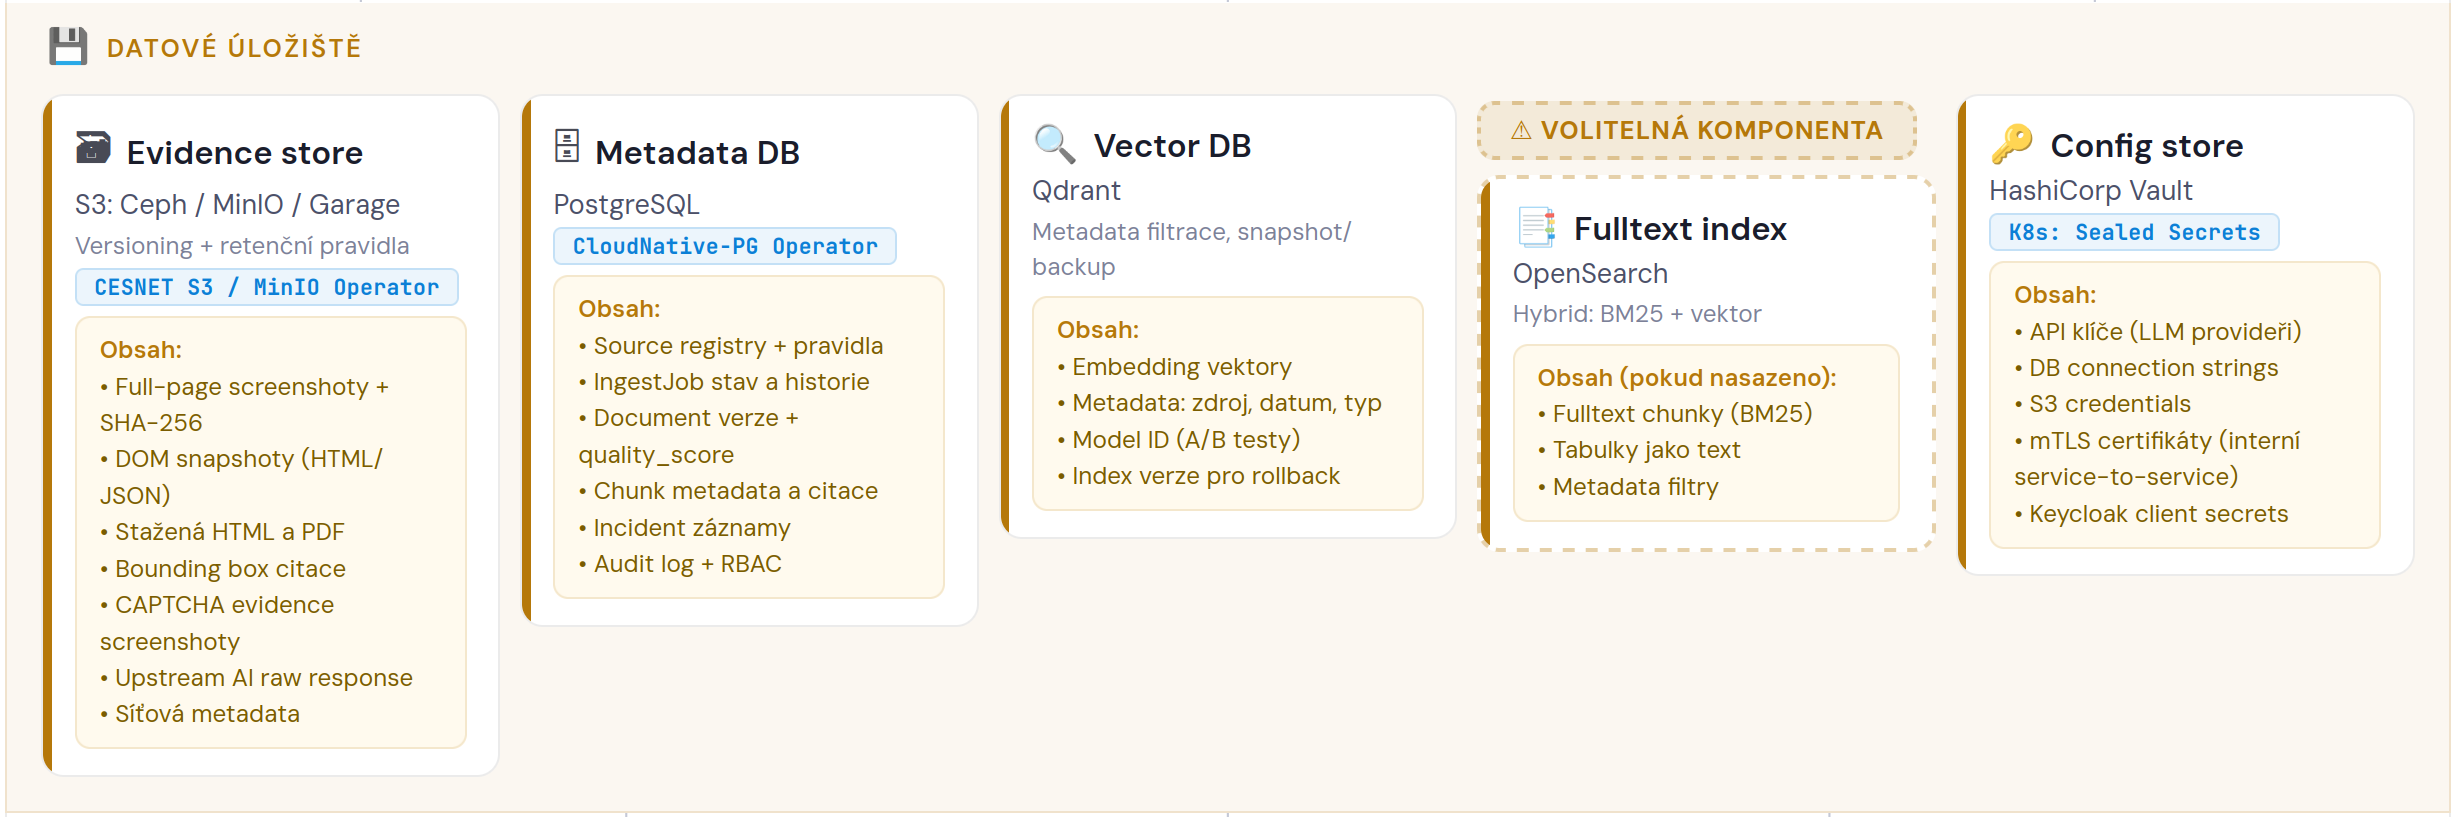
\includegraphics[width=\textwidth]{layer3.png}
\caption{Datové úložiště}
\label{fig:layer3}
\end{figure}

\newpage
\subsection{Monitoring a logy}

Monitoring bude navržen jako samostatná část infrastruktury oddělená od aplikační sítě. Prometheus~\cite{prometheus} bude sbírat číselné metriky ze všech služeb (throughput, error rate, latence, GPU utilization, queue depth). Loki~\cite{loki} bude centralizovat textové logy ze všech kontejnerů (CAPTCHA events, audit trail, error logy). Oba systémy budou definovat alert rules, které při překročení prahů budou odesílat alerty do Alertmanageru~\cite{alertmanager}.

Alertmanager bude provádět routing, grouping a~silencing alertů. Notifikace budou odesílány přes Telegram Bot API do projektového chatu. Typy alertů: ingest failure, CAPTCHA incident detected, queue backlog, DB/storage výpadek, LLM latence nad SLA, embedding worker nedostupný, error rate nad prahem.

Grafana~\cite{grafana} bude poskytovat webový dashboard pro vizualizaci stavu systému v~reálném čase s~datasources Prometheus a~Loki. Grafana Alloy~\cite{alloy} bude agent běžící na každém serveru, který bude sbírat logy a~metriky ze všech kontejnerů a~odesílat je do příslušných služeb. Schéma monitoringu je na obr.~\ref{fig:layer4}.

\begin{figure}[H]
\centering
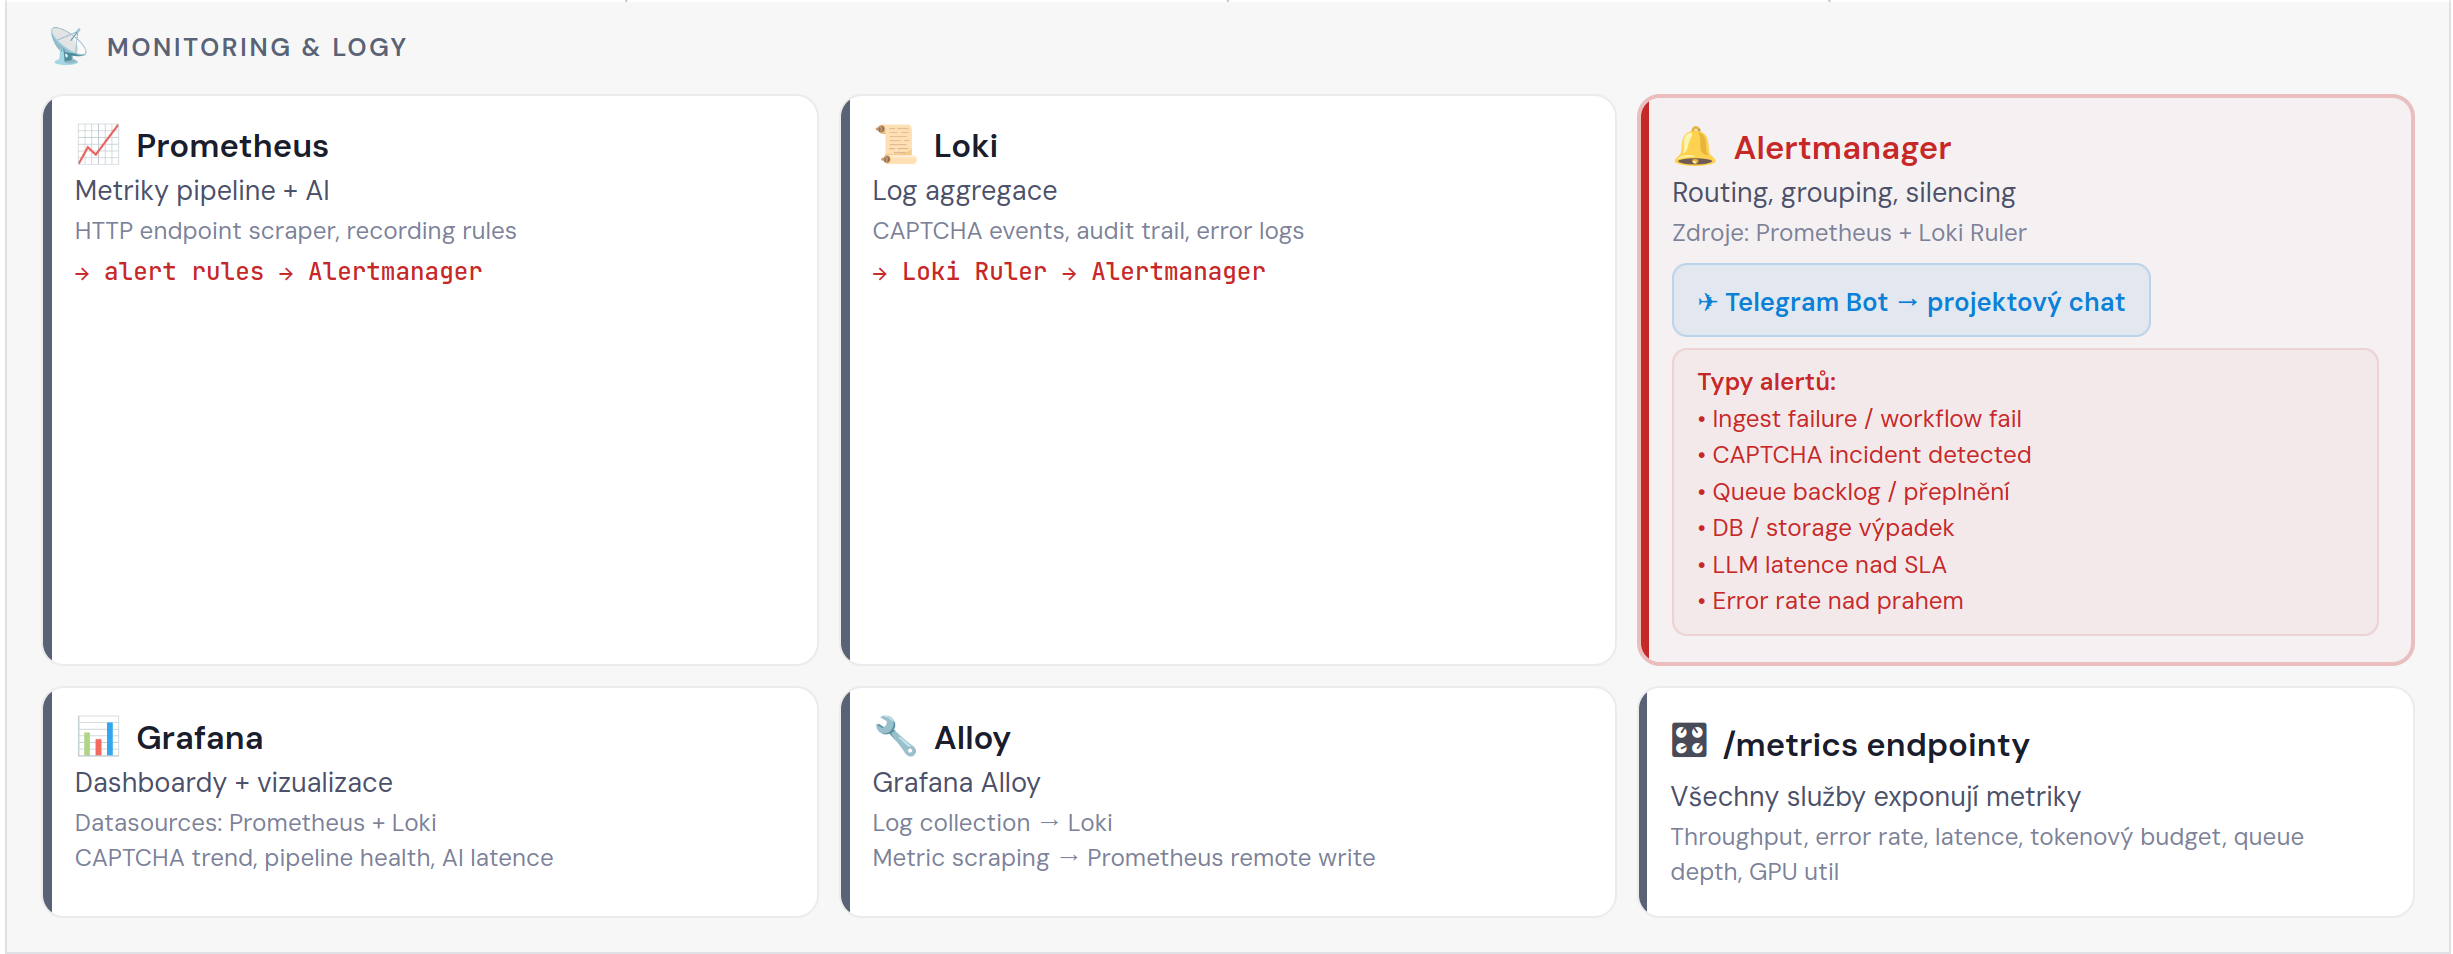
\includegraphics[width=\textwidth]{layer4.png}
\caption{Monitoring a logy}
\label{fig:layer4}
\end{figure}

\newpage
\subsection{Nasazení -- e-INFRA CZ infrastruktura}

Celý systém poběží na infrastruktuře e-INFRA CZ~\cite{einfra} -- národní výzkumné infrastruktuře pro akademickou komunitu v~ČR. Nasazení bude rozděleno do tří prostředí.

MVP (Docker~\cite{docker} Compose) poběží na virtuálním serveru v~e-INFRA CZ OpenStack~\cite{openstack} Cloud (G2 Brno / G2 Ostrava). VM s~GPU pro embedding/VLM workery. Reverse proxy: Traefik (potvrzeno). Perzistentní svazky na Ceph block storage. TLS přes cert-manager + Let's Encrypt.

Produkční Kubernetes poběží na CERIT-SC Kubernetes platformě spravované přes Rancher. Ingress: NGINX Ingress (default v~Rancher) nebo Traefik dle omezení clusteru. TLS: cert-manager s~\texttt{letsencrypt-prod} ClusterIssuer. K~dispozici: MinIO Operator pro S3, CloudNative-PG pro PostgreSQL, GPU (NVIDIA L40/L40S 48GB, T4 16GB), Harbor~\cite{harbor} (\texttt{hub.cerit.io}) jako container registry, namespace separation (core vs monitoring).

Batch a~AI výpočty poběží na MetaCentrum Grid (PBS scheduler). GPU clustery: alfrid (NVIDIA L40/L40S 48GB pro 70B Q4 modely), DGX H100 (8x H100 80GB, on-demand), T4 15GB (embedding, VLM extrakce). Výpočty poběží v~Singularity (Apptainer)~\cite{apptainer} kontejnerech s~NGC images přes CVMFS. Doplňkově CERIT-SC AIaaS (OpenAI-compatible API).

CI/CD: 13 vývojářů na GitHubu. Pipeline: build Docker images, testy (Pytest~\cite{pytest} backend, Playwright E2E), push do Harbor, kubectl deploy na K8s s~GitHub Actions~\cite{ghactions}. Volitelně mirror na \texttt{gitlab.ics.muni.cz} pro GitLab K8s Agent. Aplikace vystavené na CERIT-SC budou dostupné pod doménou \texttt{*.dyn.cloud.e-infra.cz} s~automatickou DNS registrací. Přehled nasazení je na obr.~\ref{fig:layer5}.

\begin{figure}[H]
\centering
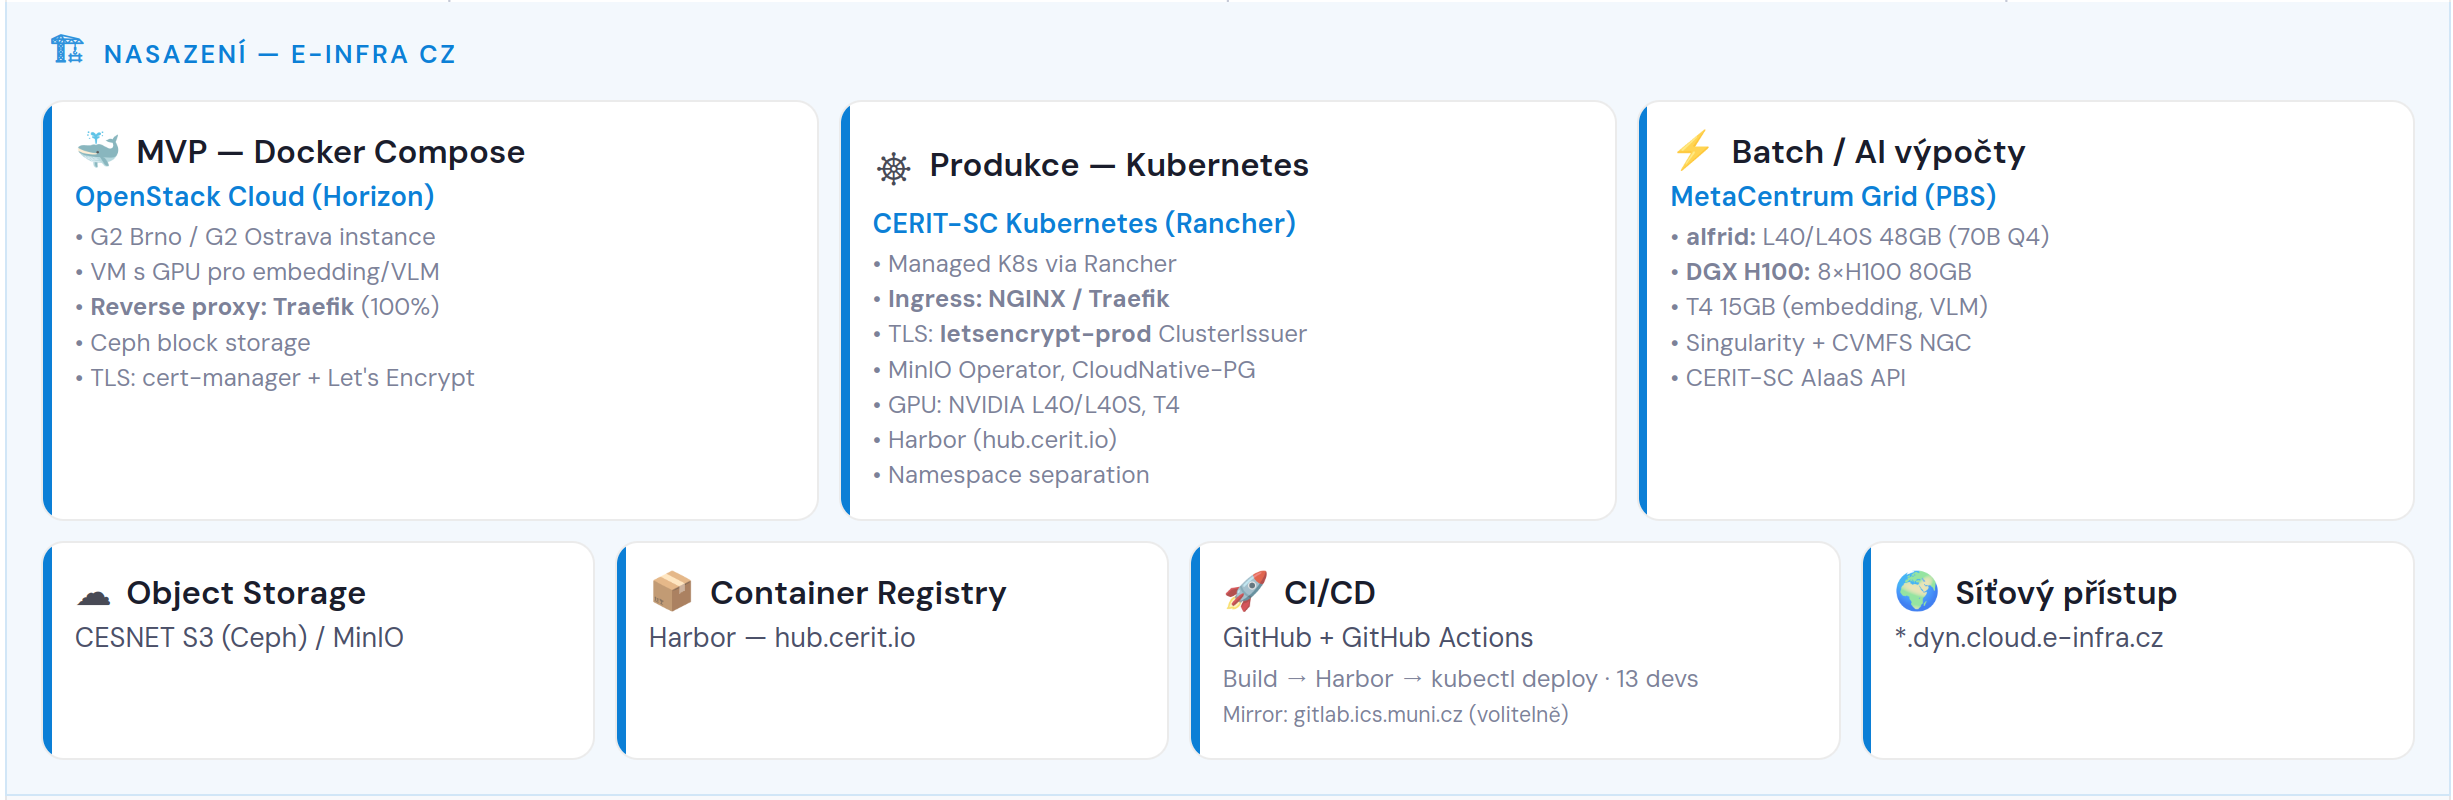
\includegraphics[width=\textwidth]{layer5.png}
\caption{Nasazení na e-INFRA CZ}
\label{fig:layer5}
\end{figure}

\newpage
% ══════════ 6. PIPELINE DIAGRAM ══════════
\section{Diagram ingest pipeline a RAG zpracování}

Pipeline diagram zobrazuje kompletní datový tok systému -- od registrace zdroje přes multimodální sběr dat až po generování odpovědí pomocí LLM. Diagram zachycuje fallback logiku mezi strategiemi sběru, quality gate pro vyhodnocení kvality obsahu, větvení při detekci CAPTCHA a~celý proces normalizace, chunkování, embeddingu a~RAG retrievalu. Celý tok dat je zachycen na obr.~\ref{fig:pipeline}.

Tok dat bude začínat v~Source Registry, kde bude evidován zdroj (URL, pravidla, licence). Orchestrátor naplánuje úlohu a~zařadí ji do fronty RabbitMQ. Worker proces odebere úlohu a~zahájí sběr dat dle preferované strategie -- nejprve API/Feed, pak HTML Fetch + Parse, Rendered DOM (Playwright), Screenshot Screening a~jako poslední Upstream AI Provider. Mezi každými dvěma strategiemi bude vyznačen fallback přechod.

Po získání obsahu budou data předána do Quality Gate -- rozhodovacího bodu, který vyhodnotí, zda je obsah dostatečně kvalitní. Pokud ano, data budou pokračovat do normalizace (Canonical Document), kde se vytvoří jednotný formát s~metadaty a~citacemi. Pokud kvalita nedostačuje, systém automaticky přejde na další strategii ve fallback řetězci.

Pokud bude při sběru detekována CAPTCHA, blokace nebo jiná chyba, vytvoří se záznam v~Incident DB s~evidencí a~zařadí se do fronty pro řešení. Po vyřešení incidentu se úloha automaticky zopakuje (retry after resolution -- přerušovaná čára zpět na začátek pipeline).

Normalizovaný dokument se uloží do Document DB a~artefakty (screenshoty, HTML, PDF, DOM) do S3 Evidence Store. Následně proběhne Chunking a~výpočet Embeddings, jejichž výsledky se uloží do Vector DB. Nad vektorovým indexem pak bude fungovat Query API / RAG Retrieval, který při dotazu uživatele vyhledá relevantní chunky a~předá je LLM modelu pro generování odpovědi s~citacemi.

\begin{figure}[H]
\centering
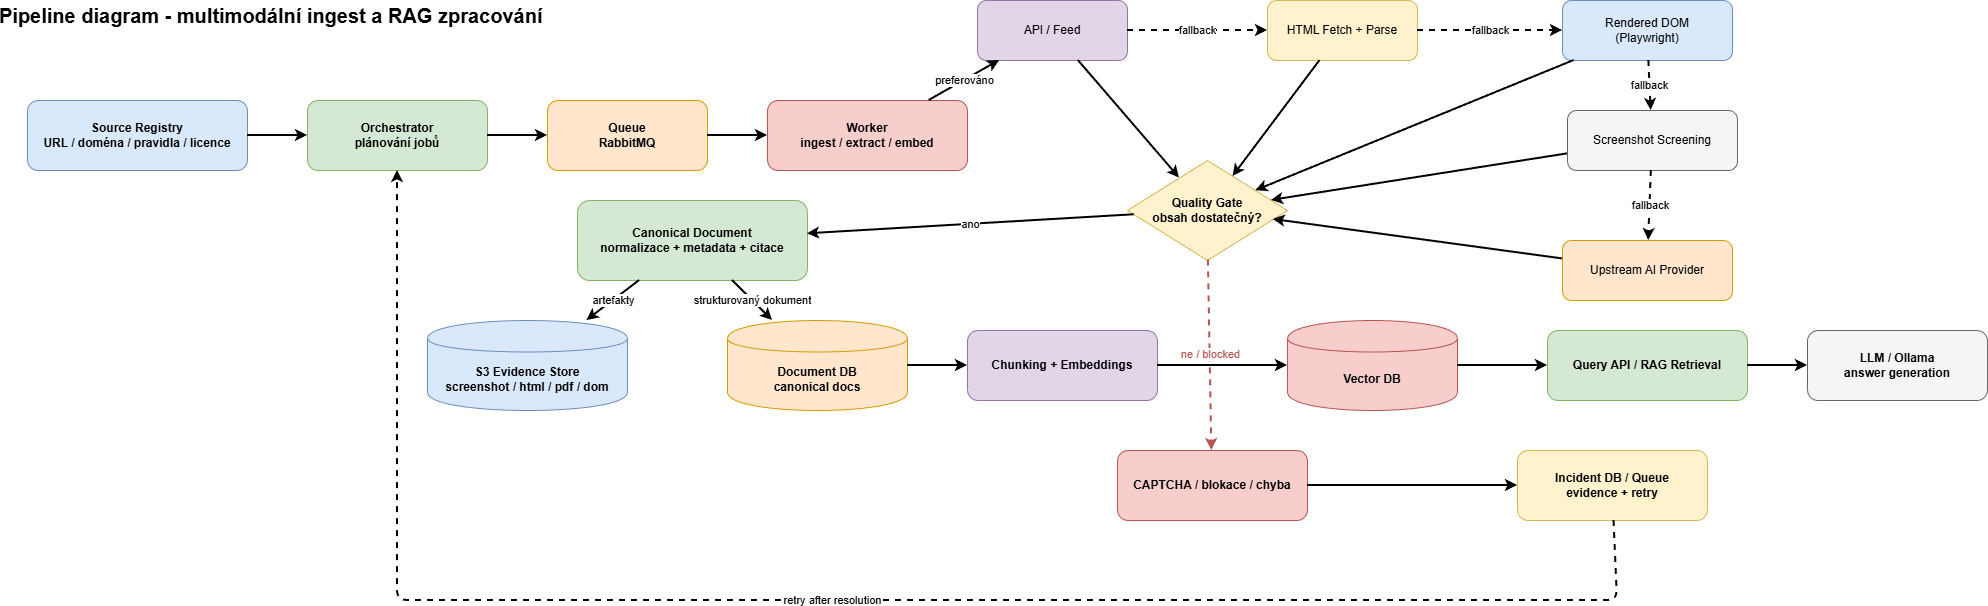
\includegraphics[width=\textwidth]{pipeline.png}
\caption{Pipeline diagram -- multimodální ingest a RAG zpracování}
\label{fig:pipeline}
\end{figure}

\newpage
% ══════════ 7. SEKVENČNÍ DIAGRAM ══════════
\section{Sekvenční diagram -- zpracování dotazu v režimu RAG}

Sekvenční diagram zachycuje průběh zpracování jednoho dotazu uživatele v~režimu RAG. Diagram zobrazuje komunikaci mezi šesti komponentami systému: Frontend (Vue + TypeScript), Backend (FastAPI), PostgreSQL (metadata a~audit), Vector DB (Qdrant), Document DB a~LLM (lokální inference engine -- llama.cpp nebo Ollama, viz sekci~\ref{sec:architektura}). Průběh zpracování je zachycen na obr.~\ref{fig:sekvencni}.

Průběh zpracování dotazu zachycený v~diagramu probíhá v~následujících krocích:

\textbf{Krok 1--2:} Uživatel zadá dotaz v~přirozeném jazyce prostřednictvím webového UI. Frontend odešle požadavek na Backend přes REST API.

\textbf{Krok 3--4:} Backend uloží dotaz a~auditní stopu do PostgreSQL databáze. Každý dotaz je zaznamenán pro účely auditu a~reprodukovatelnosti.

\textbf{Krok 5--6:} Backend provede similarity search (top-k retrieval) ve Vector DB. Vektorová databáze vrátí nejrelevantnější chunky spolu se skóre podobnosti. Vyhledávání využívá embedding dotazu porovnaný s~embeddingy uložených chunků.

\textbf{Krok 7--8:} Na základě nalezených chunků Backend načte z~Document DB plné dokumenty, metadata a~citační reference. Tím získá kontext potřebný pro sestavení odpovědi včetně evidence pro citace.

\textbf{Krok 9--10:} Backend sestaví prompt obsahující kontext (nalezené dokumenty), instrukce (formát odpovědi, požadavek na citace) a~samotný dotaz uživatele. Tento prompt odešle LLM modelu, který vygeneruje odpověď s~citacemi na zdrojové dokumenty.

\textbf{Krok 11--12:} Odpověď modelu včetně citací se uloží zpět do PostgreSQL pro pozdější dohledání a~audit.

\textbf{Krok 13--14:} Backend odešle odpověď frontendu, který ji zobrazí uživateli včetně citací. Uživatel bude moci kliknout na citaci a~zobrazit si zdrojový dokument nebo důkazní artefakt (screenshot, HTML).

Celý proces bude navržen tak, aby byl plně dohledatelný -- od zadání dotazu přes nalezené dokumenty až po vygenerovanou odpověď. Každý krok bude zaznamenán a~bude ho možné zpětně reprodukovat.

\begin{figure}[H]
\centering
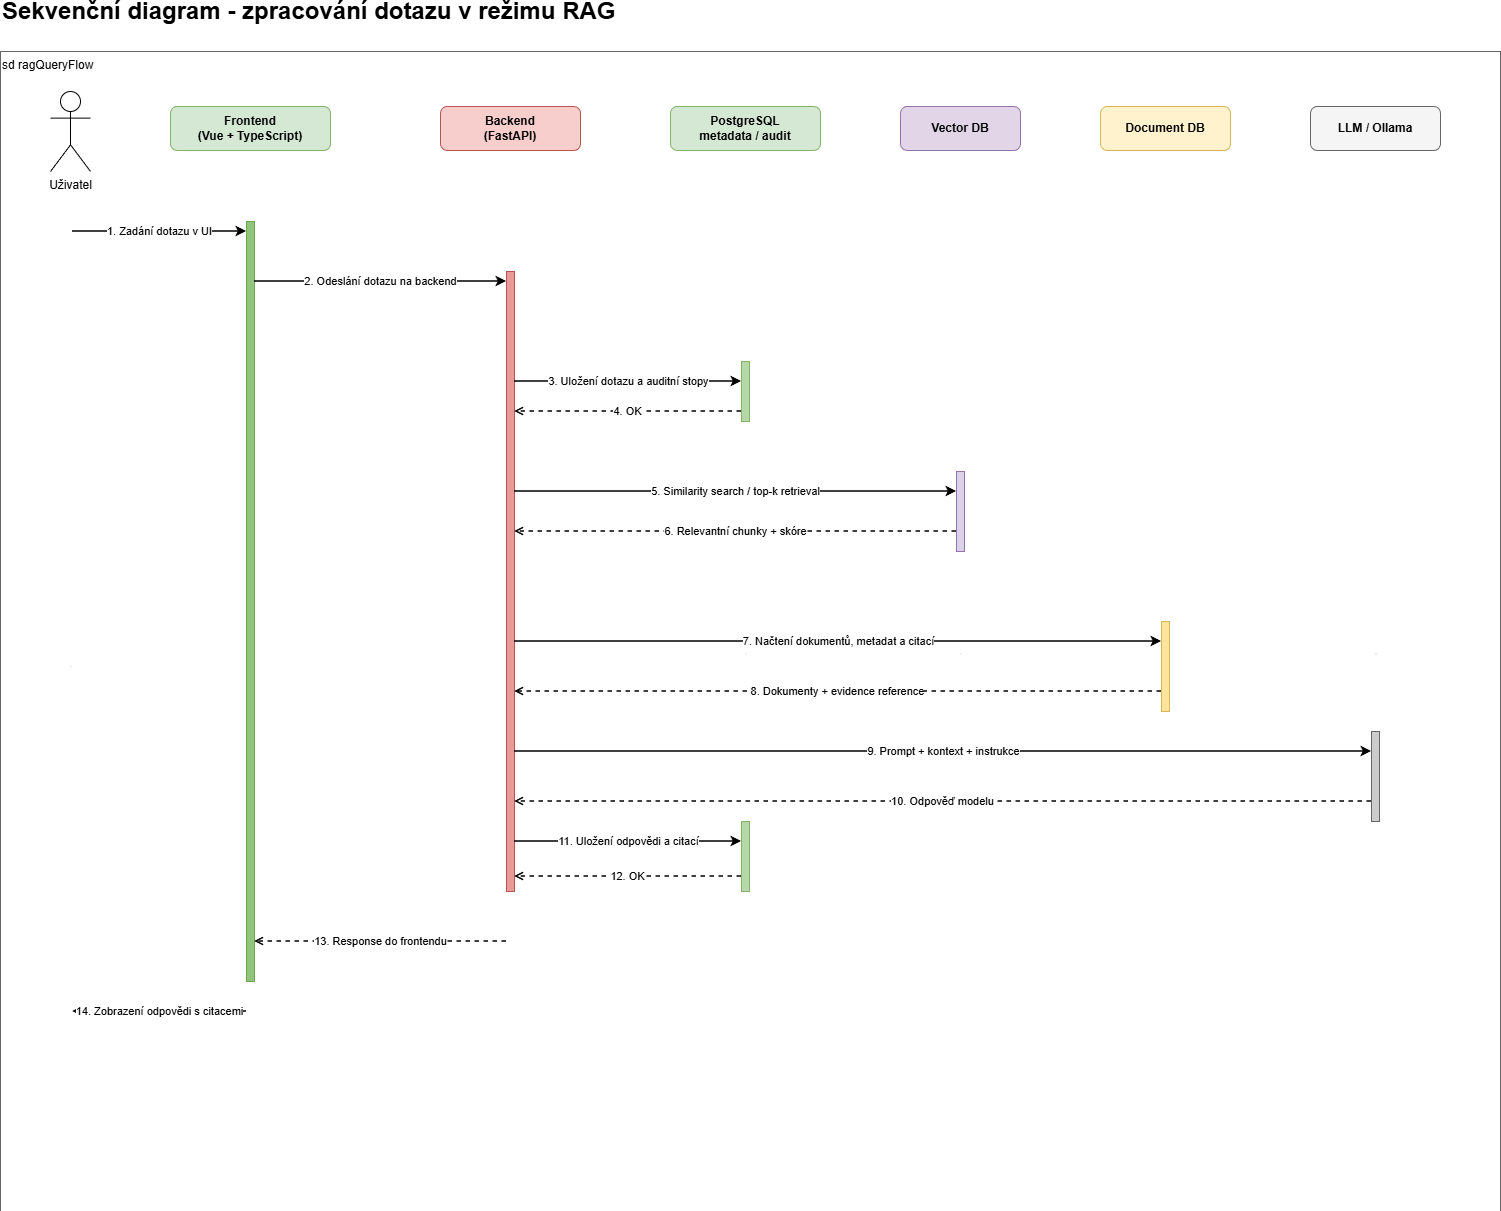
\includegraphics[width=\textwidth]{sekvencni.png}
\caption{Sekvenční diagram -- zpracování dotazu v režimu RAG}
\label{fig:sekvencni}
\end{figure}

\newpage
% ══════════ 8. ROLE ══════════
\section{Uživatelské role a řízení přístupu}

Systém bude implementovat RBAC. Autentizace bude realizována přes Keycloak s~podporou Google OAuth2 (OIDC). JWT tokeny budou řídit session management. Každá operace bude zaznamenána do auditního logu.

\textbf{Administrátor} bude mít plný přístup ke konfiguraci systému, správě uživatelů a~rolí, retenčním pravidlům, Vault tajemstvím a~řešení CAPTCHA incidentů.

\textbf{Kurátor} bude spravovat zdroje dat, nastavovat pravidla sběru, dokládat právní tituly a~řešit incidenty vzniklé při ingest pipeline.

\textbf{Analytik} bude moci provádět experimenty, testovat modely, specifikovat testovací datasety a~vyhodnocovat kvalitu indexu.

\textbf{Standardní uživatel} bude moci zadávat dotazy, volit režim dotazování (RAG/no-RAG) a~zobrazovat odpovědi s~citacemi. Přístup k~důkazním artefaktům může být omezen.

\newpage
% ══════════ 9. DATOVÝ MODEL ══════════
\section{Datový model}

Datový model bude navržen tak, aby umožňoval evidenci zdrojů dat, průběhu ingest pipeline, uložených dokumentů, embeddingů, incidentů a~auditních záznamů. Model bude podporovat verzování dokumentů, ukládání důkazních artefaktů a~dohledatelnost všech operací. ER diagram je na obr.~\ref{fig:er}.

ER diagram zobrazuje osm entit a~jejich vztahy. Centrální entitou je \textbf{Source} (zdroj dat), který definuje URL, pravidla sběru, právní titul a~retenční politiku. Každý zdroj může mít více \textbf{IngestJob} záznamů (1:N) -- každý IngestJob reprezentuje jeden pokus o~stažení dat s~evidencí použité strategie, stavu a~případného error kódu.

Ze zdroje vznikají \textbf{Document} záznamy (1:N) -- normalizované dokumenty s~verzováním a~quality score. Každý dokument se dělí na \textbf{Chunk} záznamy (1:N), přičemž chunk může být typu text, tabulka nebo layout blok. Každý chunk má jeden nebo více \textbf{Embedding} záznamů (1:N) -- vektorovou reprezentaci s~identifikací použitého modelu a~verze.

\textbf{Incident} je vázán na zdroj (1:N) a~obsahuje typ problému (např. CAPTCHA), závažnost, stav řešení a~referenci na důkazní artefakty. \textbf{Evidence} artefakty (screenshoty, HTML, PDF, DOM snapshoty) jsou propojeny s~Incident záznamy vazbou N:M (evidence\_refs) a~s~Document záznamy vazbou N:M (reference). Každý artefakt má unikátní SHA-256 hash a~URI v~objektovém úložišti.

\textbf{AuditLog} zaznamenává všechny operace v~systému a~je propojen s~entitami Source a~Document vazbou N:M (logged actions) -- umožní zpětně dohledat, kdo a~kdy provedl jakou akci nad kterým objektem.

Datový model bude navržen tak, aby bylo možné přidávat nové strategie sběru, nové modely a~nové typy dokumentů bez zásadních změn struktury databáze.

\begin{figure}[H]
\centering
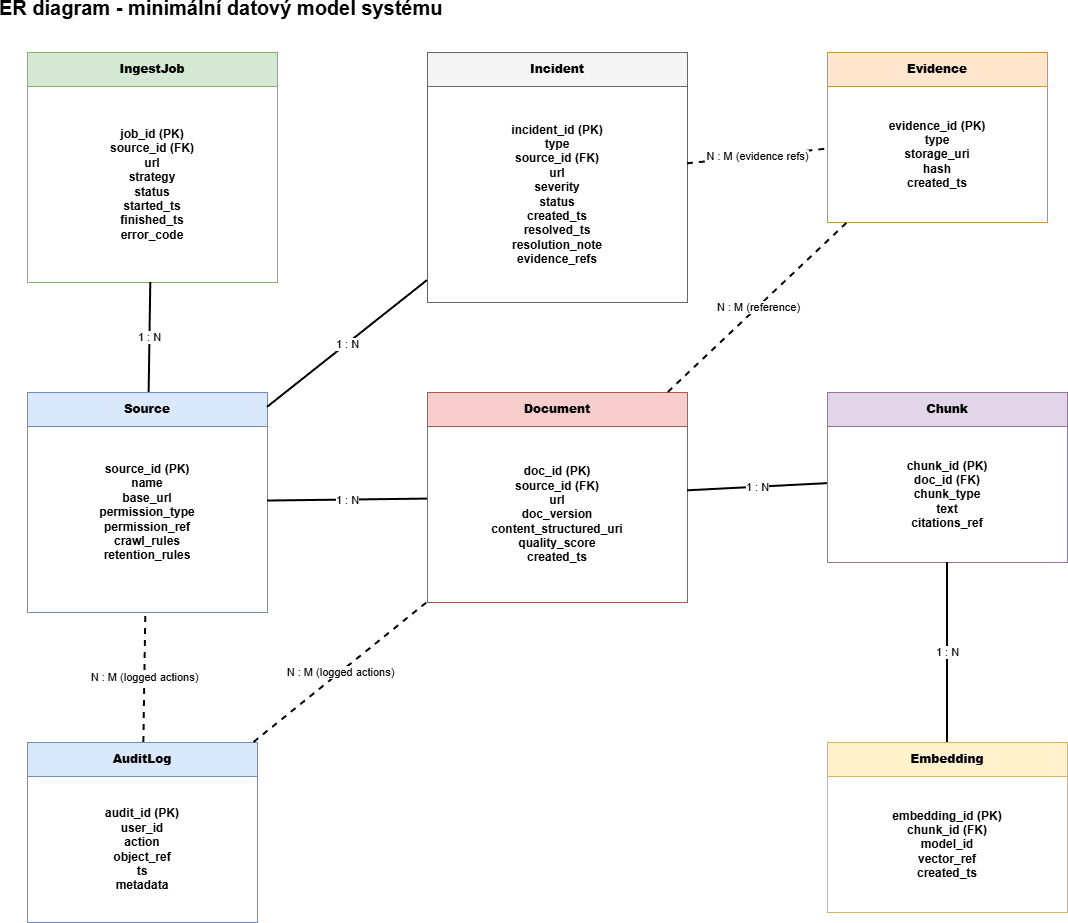
\includegraphics[width=0.85\textwidth]{er_diagram.png}
\caption{ER diagram -- minimální datový model systému}
\label{fig:er}
\end{figure}

Přehled všech entit s~jejich klíčovými atributy je v tab.~\ref{tab:entity}.

\begin{table}[H]
\centering\small
\begin{tabularx}{\textwidth}{l X}
\toprule
\textbf{Entita} & \textbf{Popis a~klíčové atributy} \\
\midrule
\texttt{Source} & Webový zdroj -- source\_id, name, base\_url, permission\_type, permission\_ref, crawl\_rules, retention\_rules \\
\addlinespace
\texttt{IngestJob} & Úloha stažení -- job\_id, source\_id, url, strategy, status, started\_ts, finished\_ts, error\_code \\
\addlinespace
\texttt{Evidence} & Důkazní artefakt -- evidence\_id, type [screenshot/html/dom/pdf], storage\_uri, hash, created\_ts \\
\addlinespace
\texttt{Document} & Zpracovaný dokument -- doc\_id, source\_id, url, doc\_version, content\_structured\_uri, quality\_score \\
\addlinespace
\texttt{Chunk} & Fragment dokumentu -- chunk\_id, doc\_id, chunk\_type [text/table/block], text, citations\_ref \\
\addlinespace
\texttt{Embedding} & Vektorová reprezentace -- embedding\_id, chunk\_id, model\_id, vector\_ref, created\_ts \\
\addlinespace
\texttt{Incident} & Problém -- incident\_id, type, source\_id, url, severity, status, resolved\_ts, resolution\_note, evidence\_refs \\
\addlinespace
\texttt{AuditLog} & Akce -- audit\_id, user\_id, action, object\_ref, ts, metadata \\
\bottomrule
\end{tabularx}
\caption{Datové entity systému}
\label{tab:entity}
\end{table}

\newpage
% ══════════ 8. BEZPEČNOST ══════════
\section{Bezpečnost, právní omezení, testování a zajištění kvality}

Pro každý zdroj dat bude muset existovat definovaný právní titul (písemné povolení, veřejně dostupný obsah, smluvní přístup). Retenční pravidla bude možné nastavit samostatně pro HTML, screenshoty, metadata a~indexy. Citlivé údaje (API klíče, tokeny) budou ukládány v~HashiCorp Vault nebo Kubernetes Sealed Secrets. Interní komunikace mezi službami bude zabezpečena mTLS certifikáty. Systém nebude implementovat obcházení ochranných mechanismů -- při detekci CAPTCHA bude vytvořen incident. Databáze a~úložiště budou připojeny pouze ke storage síti a~nebudou dostupné z~externího prostředí.

Backend bude testován pomocí Pytest (unit a~integrační testy). Frontend a~E2E testy budou používat Playwright. Smoke testy se budou spouštět při každém nasazení. Kvalita RAG odpovědí bude vyhodnocována pomocí testovacího datasetu s~metrikami Recall@k, MRR, nDCG. CI/CD: GitHub Actions automaticky při každém commitu.

\newpage
% ══════════ 10. PLÁN IMPLEMENTACE ══════════
\section{Plán implementace}

Vývoj systému je rozdělen do čtyř fází dle metodiky Unified Process (UP): Zahájení, Rozpracování, Konstrukce a~Zavedení. Každá fáze obsahuje konkrétní aktivity s~odhadovanou náročností.

\subsection{Fáze Zahájení (Inception)}

Aktivity fáze Zahájení s~odhadovanou náročností jsou v tab.~\ref{tab:plan-zahajeni}.
Tabulka zahrnuje aktivity potřebné k~ustavení projektu -- od prostudování zadání přes definici cílů až po nastavení vývojového prostředí. U~každé aktivity je uveden cílový milník a~odhadovaná časová náročnost v~hodinách.

\begin{table}[H]
\centering\small
\begin{tabularx}{\textwidth}{c X l l}
\toprule
\textbf{\#} & \textbf{Aktivita} & \textbf{Milník} & \textbf{Odhad (h)} \\
\midrule
1 & Prostudování zadání a~sestavení týmu & -- & 13 \\
2 & Definice cílů projektu a~obchodního případu & -- & 18 \\
3 & Specifikace funkčních a~nefunkčních požadavků & M0 & 20 \\
4 & Analýza rizik & M0 & 10 \\
5 & Sestavení plánu projektu a~rozdělení práce & M0 & 15 \\
6 & Nastavení vývojového prostředí a~nástrojů & M0 & 15 \\
\bottomrule
\end{tabularx}
\caption{Aktivity fáze Zahájení}
\label{tab:plan-zahajeni}
\end{table}

\subsection{Fáze Rozpracování (Elaboration)}

Aktivity fáze Rozpracování jsou shrnuty v tab.~\ref{tab:plan-rozpracovani}.
Tabulka pokrývá analytické a~návrhové aktivity, jejichž výstupem bude architektura systému, datový model, API specifikace a~testovací strategie. Fáze Rozpracování je nejnáročnější na analytickou přípravu -- správně provedená analytická fáze sníží rizika v~průběhu implementace.

\begin{table}[H]
\centering\small
\begin{tabularx}{\textwidth}{c X l l}
\toprule
\textbf{\#} & \textbf{Aktivita} & \textbf{Milník} & \textbf{Odhad (h)} \\
\midrule
7 & Specifikace případů užití & M0--M1 & 25 \\
8 & Návrh architektury systému & M0--M1 & 35 \\
9 & Datový model a~API specifikace & M0 & 30 \\
10 & Návrh modulu sběru a~zpracování dat & M1 & 20 \\
11 & Návrh AI a~RAG vrstvy & M1--M2 & 20 \\
12 & Bezpečnostní návrh a~politika dat & M0--M2 & 15 \\
13 & Testovací strategie a~akceptační kritéria & M1--M4 & 15 \\
14 & Implementace a~testování prvního prototypu & M1 & 50 \\
15 & Prezentace výstupů zahájení a~rozpracování & -- & 15 \\
\bottomrule
\end{tabularx}
\caption{Aktivity fáze Rozpracování}
\label{tab:plan-rozpracovani}
\end{table}

\subsection{Fáze Konstrukce (Construction)}

Aktivity fáze Konstrukce jsou shrnuty v tab.~\ref{tab:plan-konstrukce}.
Tabulka obsahuje implementační aktivity rozdělené podle komponent systému -- od infrastruktury přes backend pipeline až po AI vrstvu a~frontend. Tato fáze tvoří největší část hodinové náročnosti projektu a~probíhá paralelně ve více týmech.

\begin{table}[H]
\centering\small
\begin{tabularx}{\textwidth}{c X l l}
\toprule
\textbf{\#} & \textbf{Aktivita} & \textbf{Milník} & \textbf{Odhad (h)} \\
\midrule
16 & Zprovoznění infrastruktury a~prostředí & M0--M1 & 50 \\
17 & Implementace modulu sběru dat & M1 & 70 \\
18 & Implementace zpracování a~ukládání obsahu & M1 & 60 \\
19 & Implementace vektorového indexu a~RAG pipeline & M2 & 90 \\
20 & Implementace API a~UI & M2 & 80 \\
21 & Implementace autentizace, autorizace, auditování & M2 & 40 \\
22 & Nasazení monitoringu a~observability & M2 & 35 \\
23 & Evaluace a~porovnání přístupů & M3 & 80 \\
24 & Průběžná technická dokumentace & M0--M4 & 40 \\
\bottomrule
\end{tabularx}
\caption{Aktivity fáze Konstrukce}
\label{tab:plan-konstrukce}
\end{table}

\subsection{Fáze Zavedení (Transition)}

Aktivity fáze Zavedení jsou shrnuty v tab.~\ref{tab:plan-zavedeni}.
Tabulka zachycuje aktivity závěrečné fáze projektu zaměřené na evaluaci, optimalizaci, dokumentaci a~prezentaci výsledků. Zahrnuje i~rezervy pro případné opravy a~ladění systému před finálním odevzdáním.

\begin{table}[H]
\centering\small
\begin{tabularx}{\textwidth}{c X l l}
\toprule
\textbf{\#} & \textbf{Aktivita} & \textbf{Milník} & \textbf{Odhad (h)} \\
\midrule
25 & Zálohy, obnova, DR & M4 & 50 \\
26 & Bezpečnostní hardening & M4 & 40 \\
27 & Produkční nasazení a~konfigurace & M4 & 60 \\
28 & Provozní dokumentace a~příručky & M4 & 50 \\
29 & Finální testy a~akceptace systému & M4 & 50 \\
30 & Prezentace a~obhajoba & -- & 20 \\
\bottomrule
\end{tabularx}
\caption{Aktivity fáze Zavedení}
\label{tab:plan-zavedeni}
\end{table}

\subsection{Rezervy}

Na studenta jsou navíc kalkulovány rezervy: samostudium technologií (20h), dokumentace řešení (10h), vlastní testování (10h) a~komunikace a~synchronizace v~týmu (7h).

\newpage
% ══════════ 11. ANALÝZA RIZIK ══════════
\section{Analýza rizik}

\subsection{Technická rizika}

\textbf{T-01: Nízká kvalita extrakce obsahu.} RAG bude dostávat neúplná nebo chybná data, citace budou nepřesné. Mitigace: definovat kvalitativní prahy, kombinovat více metod extrakce, průběžná manuální kontrola vzorků.

\textbf{T-02: Tichá selhání při zpracování dat.} Data se tiše nezpracují, index bude neúplný, systém se bude tvářit funkčně, ale odpovědi budou zastaralé. Mitigace: alerting a~monitoring co nejvíce kroků pipeline, testy.

\textbf{T-03: Embedding worker -- výkonnostní bottleneck.} Velký backlog fronty, pomalý rebuild indexu, zpoždění milníku M2. Mitigace: asynchronní fronta úloh, dávkové zpracování, využití výpočetní kapacity MetaCentra (alfrid L40/L40S 48GB, DGX H100).

\textbf{T-04: LLM halucinace -- tvrzení bez opory v~citacích.} Výstupy systému budou nespolehlivé. Mitigace: vyžadování citací u~každé odpovědi (strict grounding), evaluace coverage citacemi, porovnání RAG vs. přímý dotaz.

\textbf{T-05: Nekonzistentní formát zpracovaného obsahu.} Degradace kvality retrieval fáze, chybné citace. Mitigace: definovat a~validovat jednotný datový formát (Canonical Document) před zahájením implementace, unit testy mapperů.

\textbf{T-06: Nestabilita komponenty pro sběr dat při dlouhém běhu.} Sběr se zastaví bez upozornění. Mitigace: restart policy, health check endpointy, monitoring spotřeby zdrojů.

\subsection{Projektová rizika}

\textbf{P-01: Nedostatečná koordinace 13členného týmu.} Duplicitní nebo nevykonaná práce, integrace nebude fungovat. Mitigace: rozdělení práce dle plánu implementace, RACI, pravidelné synchronizace, dohled manažerem projektu.

\textbf{P-02: Nedostatečná nebo opožděná dokumentace.} Nekompletní odevzdání, ztráta kontextu. Mitigace: průběžná dokumentace jako součást každé aktivity, kontrola manažerem.

\textbf{P-03: Podcenění časové náročnosti (zejména M3).} Domino efekt na M1--M4. Mitigace: prioritizovat architekturní výstupy Rozpracování před implementací, rezervovat čas v~NSS týdnech 10--11, připravit testovací dataset souběžně.

\textbf{P-04: Nedostatečné testování před odevzdáním.} Chyby těsně před deadline. Mitigace: akceptační kritéria pro každý milník, smoke test jako podmínka uzavření každé fáze.

\subsection{Bezpečnostní rizika}

\textbf{S-01: Secrets v~kódu nebo logu.} Kompromitace přihlašovacích údajů. Mitigace: pre-commit hook pro detekci secrets, konfigurační soubory mimo repozitář, HashiCorp Vault pro produkci.

\textbf{S-02: Zachycení osobních údajů třetích stran.} Porušení GDPR. Mitigace: politika zpracování dat definovaná v~M0, minimalizace ukládaných dat, automatická detekce PII.

\textbf{S-03: Neoprávněný přístup k~datům a~artefaktům.} Porušení RBAC. Mitigace: řízení přístupu na základě rolí, audit log, mTLS šifrování komunikace.

\subsection{Provozní rizika}

\textbf{O-01: Výpadek datového úložiště bez zálohy.} Ztráta zpracovaných dat. Mitigace: pravidelné zálohy s~ověřeným postupem obnovy, replikace, test obnovy v~M4.

\textbf{O-02: Absence monitoringu způsobí nepozorované selhání.} Zastaralé odpovědi bez vědomí uživatelů. Mitigace: metriky a~alerty pro každou fázi pipeline, dashboard nejpozději v~M2.

\textbf{O-03: Ztráta dat při přechodu na produkční prostředí.} Nutnost přestavby indexu. Mitigace: dokumentovaný postup migrace, export/import dat, test migrace v~M4.

\subsection{Právní rizika}

\textbf{L-01: Sběr dat bez právního titulu.} Nutnost smazat data, nelze veřejně prezentovat. Mitigace: whitelist zdrojů s~doloženým titulem povinný v~M0, kontrola robots.txt, evidence souhlasů.

\textbf{L-02: Zpracování osobních údajů bez právního základu (GDPR).} Riziko pokuty. Mitigace: minimalizace dat, krátká retenční lhůta pro citlivé zdroje, detekce osobních údajů.

\newpage
% ══════════ 12. NACENĚNÍ PROJEKTU ══════════
\section{Nacenění projektu}

Tato kapitola obsahuje finanční odhad nákladů na realizaci projektu. Nacenění vychází z~plánu implementace (kapitola 10) a~je kalkulováno na základě dohodnuté hodinové sazby 300~Kč na studenta. Odhady jsou uvedeny ve dvou variantách -- pesimistický odhad (horní hranice) a~optimistický odhad (dolní hranice, odpovídá polovině pesimistického). Nacenění používá optimistické odhady jako základ pro výpočet ceny.

\subsection{Hodinová sazba}

Pro účely nacenění byla stanovena jednotná hodinová sazba \textbf{300~Kč/h na studenta}. Tým se skládá ze 13 členů. Celková cena je kalkulována jako součin optimistického odhadu hodin a~hodinové sazby.

\subsection{Nacenění dle fází Unified Process}

\subsubsection{Fáze Zahájení (Inception)}

Nacenění aktivit fáze Zahájení je uvedeno v tab.~\ref{tab:cena-zahajeni}.
Tabulka uvádí pesimistické a~optimistické odhady hodin pro každou aktivitu fáze Zahájení spolu s~výslednou cenou v~Kč při sazbě 300~Kč/h. Optimistický odhad odpovídá přibližně polovině pesimistického a~slouží jako základ pro kalkulaci.

\begin{table}[H]
\centering\small
\begin{tabularx}{\textwidth}{c X r r r}
\toprule
\textbf{\#} & \textbf{Aktivita} & \textbf{Pesim. (h)} & \textbf{Optim. (h)} & \textbf{Cena (Kč)} \\
\midrule
1 & Prostudování zadání a~sestavení týmu & 13 & 6,5 & 1\,950 \\
2 & Definice cílů projektu a~obchodního případu & 18 & 9 & 2\,700 \\
3 & Specifikace funkčních a~nefunkčních požadavků & 20 & 10 & 3\,000 \\
4 & Analýza rizik & 10 & 5 & 1\,500 \\
5 & Sestavení plánu projektu a~rozdělení práce & 15 & 7,5 & 2\,250 \\
6 & Nastavení vývojového prostředí a~nástrojů & 15 & 7,5 & 2\,250 \\
\midrule
& \textbf{Mezisoučet -- Zahájení} & \textbf{91} & \textbf{45,5} & \textbf{13\,650} \\
\bottomrule
\end{tabularx}
\caption{Nacenění fáze Zahájení}
\label{tab:cena-zahajeni}
\end{table}

\subsubsection{Fáze Rozpracování (Elaboration)}

Nacenění aktivit fáze Rozpracování je uvedeno v tab.~\ref{tab:cena-rozpracovani}.
Tabulka zachycuje nákladově nejnáročnější analytické aktivity -- zejména návrh architektury a~datového modelu. Celková cena fáze Rozpracování odráží hloubku přípravy nutné pro úspěšnou implementaci.

\begin{table}[H]
\centering\small
\begin{tabularx}{\textwidth}{c X r r r}
\toprule
\textbf{\#} & \textbf{Aktivita} & \textbf{Pesim. (h)} & \textbf{Optim. (h)} & \textbf{Cena (Kč)} \\
\midrule
7 & Specifikace případů užití & 25 & 12,5 & 3\,750 \\
8 & Návrh architektury systému & 35 & 17,5 & 5\,250 \\
9 & Datový model a~API specifikace & 30 & 15 & 4\,500 \\
10 & Návrh modulu sběru a~zpracování dat & 20 & 10 & 3\,000 \\
11 & Návrh AI a~RAG vrstvy & 20 & 10 & 3\,000 \\
12 & Bezpečnostní návrh a~politika dat & 15 & 7,5 & 2\,250 \\
13 & Testovací strategie a~akceptační kritéria & 15 & 7,5 & 2\,250 \\
14 & Implementace a~testování prvního prototypu & 50 & 25 & 7\,500 \\
15 & Prezentace výstupů zahájení a~rozpracování & 15 & 7,5 & 2\,250 \\
\midrule
& \textbf{Mezisoučet -- Rozpracování} & \textbf{225} & \textbf{112,5} & \textbf{33\,750} \\
\bottomrule
\end{tabularx}
\caption{Nacenění fáze Rozpracování}
\label{tab:cena-rozpracovani}
\end{table}

\subsubsection{Fáze Konstrukce (Construction)}

Nacenění aktivit fáze Konstrukce je uvedeno v tab.~\ref{tab:cena-konstrukce}.
Tabulka ukazuje rozložení implementačních nákladů napříč komponentami systému. Fáze Konstrukce tvoří největší podíl celkového rozpočtu projektu a~zahrnuje veškeré práce od zprovoznění infrastruktury až po evaluaci přístupů.

\begin{table}[H]
\centering\small
\begin{tabularx}{\textwidth}{c X r r r}
\toprule
\textbf{\#} & \textbf{Aktivita} & \textbf{Pesim. (h)} & \textbf{Optim. (h)} & \textbf{Cena (Kč)} \\
\midrule
16 & Zprovoznění infrastruktury a~prostředí & 50 & 25 & 7\,500 \\
17 & Implementace modulu sběru dat & 70 & 35 & 10\,500 \\
18 & Implementace zpracování a~ukládání obsahu & 60 & 30 & 9\,000 \\
19 & Implementace vektorového indexu a~RAG pipeline & 90 & 45 & 13\,500 \\
20 & Implementace API a~UI & 80 & 40 & 12\,000 \\
21 & Implementace autentizace, autorizace, auditování & 40 & 20 & 6\,000 \\
22 & Nasazení monitoringu a~observability & 35 & 17,5 & 5\,250 \\
23 & Evaluace a~porovnání přístupů & 80 & 40 & 12\,000 \\
24 & Průběžná technická dokumentace & 40 & 20 & 6\,000 \\
\midrule
& \textbf{Mezisoučet -- Konstrukce} & \textbf{545} & \textbf{272,5} & \textbf{81\,750} \\
\bottomrule
\end{tabularx}
\caption{Nacenění fáze Konstrukce}
\label{tab:cena-konstrukce}
\end{table}

\subsubsection{Fáze Zavedení (Transition)}

Nacenění aktivit fáze Zavedení je uvedeno v tab.~\ref{tab:cena-zavedeni}.
Tabulka shrnuje náklady na evaluaci, dokumentaci a~prezentaci výsledků v~závěrečné fázi projektu. Aktivity jsou navrženy tak, aby ověřily funkčnost systému a~připravily podklady pro odevzdání.

\begin{table}[H]
\centering\small
\begin{tabularx}{\textwidth}{c X r r r}
\toprule
\textbf{\#} & \textbf{Aktivita} & \textbf{Pesim. (h)} & \textbf{Optim. (h)} & \textbf{Cena (Kč)} \\
\midrule
25 & Zálohy, obnova, DR & 50 & 25 & 7\,500 \\
26 & Bezpečnostní hardening & 40 & 20 & 6\,000 \\
27 & Produkční nasazení a~konfigurace & 60 & 30 & 9\,000 \\
28 & Provozní dokumentace a~příručky & 50 & 25 & 7\,500 \\
29 & Finální testy a~akceptace systému & 50 & 25 & 7\,500 \\
30 & Prezentace a~obhajoba & 20 & 10 & 3\,000 \\
\midrule
& \textbf{Mezisoučet -- Zavedení} & \textbf{270} & \textbf{135} & \textbf{40\,500} \\
\bottomrule
\end{tabularx}
\caption{Nacenění fáze Zavedení}
\label{tab:cena-zavedeni}
\end{table}

\subsection{Rezervy}

Kromě přímých aktivit jsou kalkulovány rezervy na podpůrné činnosti, které nelze jednoznačně přiřadit k~jednotlivým aktivitám. Rezervy jsou stanoveny na studenta a~následně přepočteny na celý tým (13 členů). Optimistický odhad odpovídá polovině pesimistického. Přehled rezerv je v tab.~\ref{tab:cena-rezervy}.

\begin{table}[H]
\centering\small
\begin{tabularx}{\textwidth}{X r r r r}
\toprule
\textbf{Typ rezervy} & \textbf{Na studenta (h)} & \textbf{Pesim. (h)} & \textbf{Optim. (h)} & \textbf{Cena (Kč)} \\
\midrule
Samostudium technologií & 20 & 260 & 130 & 39\,000 \\
Dokumentace řešení & 10 & 130 & 65 & 19\,500 \\
Vlastní testování & 10 & 130 & 65 & 19\,500 \\
Komunikace a~synchronizace & 7 & 91 & 45,5 & 13\,650 \\
\midrule
\textbf{Mezisoučet -- Rezervy} & \textbf{47} & \textbf{611} & \textbf{305,5} & \textbf{91\,650} \\
\bottomrule
\end{tabularx}
\caption{Nacenění rezerv}
\label{tab:cena-rezervy}
\end{table}

\subsection{Celkový souhrn nacenění}

Celkový souhrn nákladů projektu je v tab.~\ref{tab:cena-souhrn}.
Tabulka sumarizuje celkové náklady projektu rozdělené podle fází a~kategorií. Závěrečný součet vychází z~optimistických odhadů pracnosti a~slouží jako podklad pro smluvní ujednání.

\begin{table}[H]
\centering
\begin{tabularx}{\textwidth}{X r r r}
\toprule
\textbf{Položka} & \textbf{Pesim. (h)} & \textbf{Optim. (h)} & \textbf{Cena (Kč)} \\
\midrule
Fáze Zahájení (Inception) & 91 & 45,5 & 13\,650 \\
Fáze Rozpracování (Elaboration) & 225 & 112,5 & 33\,750 \\
Fáze Konstrukce (Construction) & 545 & 272,5 & 81\,750 \\
Fáze Zavedení (Transition) & 270 & 135 & 40\,500 \\
\midrule
\textbf{Aktivity celkem} & \textbf{1\,131} & \textbf{565,5} & \textbf{169\,650} \\
\addlinespace
Rezervy (13 studentů $\times$ 47~h) & 611 & 305,5 & 91\,650 \\
\midrule
\textbf{Projekt celkem} & \textbf{1\,742} & \textbf{871} & \textbf{261\,300} \\
\bottomrule
\end{tabularx}
\caption{Celkový souhrn nacenění projektu}
\label{tab:cena-souhrn}
\end{table}

\subsection{Poznámky k~nacenění}

Nacenění je kalkulováno na základě \textbf{optimistických odhadů} pracnosti (dolní hranice). Pesimistické odhady představují horní hranici a~jsou uvedeny pro účely plánování rizik -- skutečná pracnost se očekává mezi oběma hodnotami.

Hodinová sazba 300~Kč/h odpovídá dohodnuté sazbě pro studentské projekty. V~případě komerčního nasazení by sazba reflektovala tržní ceny, které jsou výrazně vyšší.

Nacenění nezahrnuje náklady na infrastrukturu (e-INFRA CZ je poskytována akademické komunitě bezplatně), licence komerčních AI služeb (Anthropic, Google AI Studio, OpenAI -- tyto náklady závisí na objemu využití a~jsou hrazeny zvlášť) ani případné náklady na doménová jména nebo certifikáty (Let's Encrypt je bezplatný).

Největší podíl nákladů na aktivitách bude tvořit fáze Konstrukce (48\,\% hodin aktivit), což odpovídá charakteru projektu -- jedná se o~implementačně náročný systém s~více komponentami. Rezervy budou představovat 35\,\% celkového objemu hodin a~budou reflektovat nutnost samostudia nových technologií (AI modely, vektorové databáze, multimodální extrakce), průběžné dokumentace a~koordinace ve velkém třináctičlenném týmu.

\newpage
% ══════════ 13. UPOZORNĚNÍ ══════════
\section{Upozornění k verzi dokumentu}

Tento dokument představuje návrh architektury systému ve fázi \textbf{Elaboration} dle metodiky \textbf{UP}. V~této fázi je architektura rozpracována do detailu umožňujícího zahájení implementace, avšak nejedná se o~finální verzi návrhu.

V průběhu dalších fází vývoje (Construction, Transition) mohou nastat dílčí architektonické změny, včetně případných úprav technologického stacku -- například volba konkrétní verze LLM modelu, úprava embedding pipeline, náhrada dílčích komponent na základě výsledků prototypování a~experimentů, úpravy deployment strategie na základě zkušeností s~e-INFRA CZ infrastrukturou (omezení Rancher, dostupnost GPU, kvóty), rozšíření nebo zúžení funkcionality na základě zpětné vazby od zákazníka a~upřesnění datového modelu na základě reálných dat a~integračních testů.

Architektura je navržena modulárně právě proto, aby tyto změny byly proveditelné bez zásadní restrukturalizace celého systému.

Vzhledem k~časovému rozsahu projektu (jeden semestr, 13 členů týmu) je vývojový tým oprávněn neimplementovat kompletní systém v~plném rozsahu této specifikace. Tým se zavazuje dodat funkční MVP odpovídající milníkům M0--M2. Milníky M3 (evaluace) a~M4 (hardening) budou realizovány v~rozsahu, který umožní zbývající čas semestru.

\newpage
% ══════════ ZDROJE ══════════
\renewcommand{\refname}{Zdroje}
\addcontentsline{toc}{section}{Zdroje}
\begin{thebibliography}{99}

\bibitem{vuejs} Vue.js Team, 2025. \textit{Vue 3: The Progressive JavaScript Framework} [online]. [cit. 2026-03-09]. Dostupné z: \docurl{https://vuejs.org/guide/introduction.html}

\bibitem{typescript} Microsoft, 2025. \textit{TypeScript: JavaScript With Syntax For Types} [online]. [cit. 2026-03-09]. Dostupné z: \docurl{https://www.typescriptlang.org/docs/}

\bibitem{fastapi} Ramírez, S., 2025. \textit{FastAPI} [online]. [cit. 2026-03-10]. Dostupné z: \docurl{https://fastapi.tiangolo.com/}

\bibitem{python} Python Software Foundation, 2025. \textit{Python 3 Documentation} [online]. [cit. 2026-03-06]. Dostupné z: \docurl{https://docs.python.org/3/}

\bibitem{keycloak} Red Hat, Inc., 2025. \textit{Keycloak Documentation} [online]. [cit. 2026-03-10]. Dostupné z: \docurl{https://www.keycloak.org/documentation}

\bibitem{oauth2proxy} oauth2-proxy Contributors, 2025. \textit{oauth2-proxy} [online]. [cit. 2026-03-14]. Dostupné z: \docurl{https://github.com/oauth2-proxy/oauth2-proxy}

\bibitem{traefik} Traefik Labs, 2025. \textit{Traefik Documentation} [online]. [cit. 2026-03-13]. Dostupné z: \docurl{https://doc.traefik.io/traefik/}

\bibitem{nginxingress} Kubernetes Authors, 2025. \textit{NGINX Ingress Controller} [online]. [cit. 2026-03-13]. Dostupné z: \docurl{https://kubernetes.github.io/ingress-nginx/}

\bibitem{certmanager} cert-manager Authors, 2025. \textit{cert-manager Documentation} [online]. [cit. 2026-03-13]. Dostupné z: \docurl{https://cert-manager.io/docs/}

\bibitem{prefect} Prefect Technologies, Inc., 2025. \textit{Prefect Documentation} [online]. [cit. 2026-03-14]. Dostupné z: \docurl{https://docs.prefect.io/}

\bibitem{rabbitmq} Broadcom Inc., 2025. \textit{RabbitMQ Documentation} [online]. [cit. 2026-03-08]. Dostupné z: \docurl{https://www.rabbitmq.com/docs}

\bibitem{playwright} Microsoft, 2025. \textit{Playwright for Python} [online]. [cit. 2026-03-14]. Dostupné z: \docurl{https://playwright.dev/python/docs/intro}

\bibitem{qwen25vl} Alibaba Cloud, 2025. \textit{Qwen2.5-VL-7B-Instruct} [online]. [cit. 2026-03-15]. Dostupné z: \docurl{https://huggingface.co/Qwen/Qwen2.5-VL-7B-Instruct}

\bibitem{bgem3} BAAI, 2024. \textit{BGE-M3: Multi-Functionality, Multi-Linguality, Multi-Granularity Text Embeddings} [online]. [cit. 2026-03-07]. Dostupné z: \docurl{https://huggingface.co/BAAI/bge-m3}

\bibitem{llamacpp} Gerganov, G. a~kol., 2025. \textit{llama.cpp} [online]. [cit. 2026-03-12]. Dostupné z: \docurl{https://github.com/ggerganov/llama.cpp}

\bibitem{ollama} Ollama, 2025. \textit{Ollama} [online]. [cit. 2026-03-15]. Dostupné z: \docurl{https://ollama.com}

\bibitem{llama33} Meta Platforms, Inc., 2024. \textit{Llama-3.3-70B-Instruct} [online]. [cit. 2026-03-12]. Dostupné z: \docurl{https://huggingface.co/meta-llama/Llama-3.3-70B-Instruct}

\bibitem{qwen2572b} Alibaba Cloud, 2025. \textit{Qwen2.5-72B-Instruct} [online]. [cit. 2026-03-15]. Dostupné z: \docurl{https://huggingface.co/Qwen/Qwen2.5-72B-Instruct}

\bibitem{mistralsmall} Mistral AI, 2025. \textit{Mistral-Small-3.1-24B-Instruct-2503} [online]. [cit. 2026-03-20]. Dostupné z: \docurl{https://huggingface.co/mistralai/Mistral-Small-3.1-24B-Instruct-2503}

\bibitem{anthropic} Anthropic, 2025. \textit{Anthropic API Documentation} [online]. [cit. 2026-03-16]. Dostupné z: \docurl{https://docs.anthropic.com/}

\bibitem{googleai} Google LLC, 2025. \textit{Google AI for Developers: Gemini API} [online]. [cit. 2026-03-17]. Dostupné z: \docurl{https://ai.google.dev/gemini-api/docs/ai-studio-quickstart}

\bibitem{openai} OpenAI, 2025. \textit{OpenAI Platform Documentation} [online]. [cit. 2026-03-16]. Dostupné z: \docurl{https://platform.openai.com/docs}

\bibitem{postgresql} The PostgreSQL Global Development Group, 2025. \textit{PostgreSQL Documentation} [online]. [cit. 2026-03-06]. Dostupné z: \docurl{https://www.postgresql.org/docs/}

\bibitem{qdrant} Qdrant Solutions GmbH, 2025. \textit{Qdrant Documentation} [online]. [cit. 2026-03-10]. Dostupné z: \docurl{https://qdrant.tech/documentation/}

\bibitem{opensearch} OpenSearch Contributors, 2025. \textit{OpenSearch Documentation} [online]. [cit. 2026-03-17]. Dostupné z: \docurl{https://opensearch.org/docs/latest/}

\bibitem{minio} MinIO, Inc., 2025. \textit{MinIO Documentation} [online]. [cit. 2026-03-11]. Dostupné z: \docurl{https://min.io/docs/minio/linux/index.html}

\bibitem{vault} HashiCorp, 2025. \textit{Vault Documentation} [online]. [cit. 2026-03-16]. Dostupné z: \docurl{https://developer.hashicorp.com/vault/docs}

\bibitem{prometheus} The Prometheus Authors, 2025. \textit{Prometheus Documentation} [online]. [cit. 2026-03-18]. Dostupné z: \docurl{https://prometheus.io/docs/}

\bibitem{grafana} Grafana Labs, 2025. \textit{Grafana Documentation} [online]. [cit. 2026-03-18]. Dostupné z: \docurl{https://grafana.com/docs/grafana/latest/}

\bibitem{loki} Grafana Labs, 2025. \textit{Grafana Loki Documentation} [online]. [cit. 2026-03-19]. Dostupné z: \docurl{https://grafana.com/docs/loki/latest/}

\bibitem{alertmanager} The Prometheus Authors, 2025. \textit{Alertmanager Documentation} [online]. [cit. 2026-03-19]. Dostupné z: \docurl{https://prometheus.io/docs/alerting/latest/alertmanager/}

\bibitem{alloy} Grafana Labs, 2025. \textit{Grafana Alloy Documentation} [online]. [cit. 2026-03-19]. Dostupné z: \docurl{https://grafana.com/docs/alloy/latest/}

\bibitem{docker} Docker, Inc., 2025. \textit{Docker Documentation} [online]. [cit. 2026-03-05]. Dostupné z: \docurl{https://docs.docker.com/}

\bibitem{kubernetes} The Kubernetes Authors, 2025. \textit{Kubernetes Documentation} [online]. [cit. 2026-03-05]. Dostupné z: \docurl{https://kubernetes.io/docs/}

\bibitem{rancher} SUSE, 2025. \textit{Rancher Documentation} [online]. [cit. 2026-03-11]. Dostupné z: \docurl{https://ranchermanager.docs.rancher.com/}

\bibitem{harbor} The Harbor Authors, 2025. \textit{Harbor Documentation} [online]. [cit. 2026-03-12]. Dostupné z: \docurl{https://goharbor.io/docs/}

\bibitem{apptainer} Apptainer Project, 2025. \textit{Apptainer Documentation} [online]. [cit. 2026-03-17]. Dostupné z: \docurl{https://apptainer.org/docs/user/latest/}

\bibitem{ghactions} GitHub, Inc., 2025. \textit{GitHub Actions Documentation} [online]. [cit. 2026-03-08]. Dostupné z: \docurl{https://docs.github.com/en/actions}

\bibitem{pytest} pytest-dev team, 2025. \textit{pytest Documentation} [online]. [cit. 2026-03-08]. Dostupné z: \docurl{https://docs.pytest.org/}

\bibitem{playwrighttest} Microsoft, 2025. \textit{Playwright} [online]. [cit. 2026-03-14]. Dostupné z: \docurl{https://playwright.dev/docs/intro}

\bibitem{einfra} CESNET, z.~s.~p.~o., 2025. \textit{e-INFRA CZ Documentation} [online]. [cit. 2026-03-06]. Dostupné z: \docurl{https://docs.e-infra.cz/}

\bibitem{openstack} e-INFRA CZ, 2025. \textit{Cloud -- e-INFRA CZ Documentation} [online]. [cit. 2026-03-06]. Dostupné z: \docurl{https://docs.platforms.cloud.e-infra.cz/en/docs}

\bibitem{ceritk8s} CERIT-SC, 2025. \textit{CERIT-SC Platform Overview} [online]. [cit. 2026-03-11]. Dostupné z: \docurl{https://docs.cerit.io/en/docs/platform/overview}

\bibitem{metacentrum} CESNET, z.~s.~p.~o., 2025. \textit{MetaCentrum Documentation} [online]. [cit. 2026-03-07]. Dostupné z: \docurl{https://docs.metacentrum.cz}

\bibitem{ceritaiaas} CERIT-SC, 2025. \textit{AI as a Service -- CERIT-SC} [online]. [cit. 2026-03-20]. Dostupné z: \docurl{https://docs.cerit.io/en/docs/ai-as-a-service/ai-api}

\bibitem{cesnets3} CESNET, z.~s.~p.~o., 2025. \textit{Object Storage S3 -- CESNET DU} [online]. [cit. 2026-03-07]. Dostupné z: \docurl{https://docs.du.cesnet.cz/en/docs/object-storage-s3/s3-service}

\end{thebibliography}

\end{document}
